\documentclass[a4paper,11pt]{report}
\usepackage{fullpage}

\usepackage[latin1]{inputenc}
\usepackage[T1]{fontenc}

\renewcommand*\rmdefault{ppl}

% Choix de la langue
\usepackage[english]{babel}
%\selectlanguage{francais} % fran�ais
%\selectlanguage{english} % english

%math
\usepackage{extpfeil}
\usepackage{stmaryrd,amsfonts,latexsym,url,amsmath,amssymb,amsthm,amscd,mathtools}
\usepackage{multirow}
\usepackage{ebproof}
%\usepackage{mathrsfs}

\usepackage{newtxmath}
\usepackage{newtxtext}
\usepackage{lmodern}
\rmfamily

%figures
%\usepackage{subfig}
\usepackage{caption}
\usepackage{subcaption}
\usepackage{graphicx}
\usepackage{xargs} % Use more than one optional parameter in a new commands
\usepackage[pdftex,dvipsnames]{xcolor}
\usepackage{tikz}
\usetikzlibrary{matrix,arrows,decorations.pathmorphing}
\usetikzlibrary{shapes}
\usetikzlibrary{calc}
\usetikzlibrary{arrows.meta}
\usepackage{wrapfig}

\usepackage[colorlinks=true, citecolor=purple, linkcolor = blue]{hyperref}

\usepackage{pdflscape}

\usepackage{mdframed}
%% Todo notes
%\usepackage[colorinlistoftodos,prependcaption,textsize=tiny]{todonotes}
\usepackage[colorinlistoftodos,prependcaption]{todonotes}
\newcommandx{\unsure}[2][1=]{\todo[linecolor=red,backgroundcolor=red!25,bordercolor=red,#1]{#2}}
\newcommandx{\change}[2][1=]{\todo[linecolor=blue,backgroundcolor=blue!25,bordercolor=blue,#1]{#2}}
\newcommandx{\info}[2][1=]{\todo[linecolor=OliveGreen,backgroundcolor=OliveGreen!25,bordercolor=OliveGreen,#1]{#2}}
\newcommandx{\improvement}[2][1=]{\todo[linecolor=Plum,backgroundcolor=Plum!25,bordercolor=Plum,#1]{#2}}
\newcommandx{\thiswillnotshow}[2][1=]{\todo[disable,#1]{#2}}

%% Arrows
\newcommand{\fw}{\mathrel{\longrightarrow}} % Forward
\newcommand{\bw}{\mathrel{\rightsquigarrow}} % Backward
\newcommand{\fbw}{\mathrel{\twoheadrightarrow}} % Forward or backward
\newcommand{\red}{\mathrel{\fw}}
\newcommand{\redl}[1]{\mathrel{\xrightarrow{#1}}}
\newcommand{\revredl}[1]{\mathrel{\xrsa{#1}}}
\newcommand{\fbl}[1]{\mathrel{\xrightarrow{#1}}}
\newcommand{\wred}{\ensuremath{\Rightarrow}}
\newcommand{\wredl}[1]{\mathrel{\overset{#1}{\wred}}}


%order relations
\newcommand{\substeq}{\ensuremath{\sqsubseteq}}
\newcommand{\subst}{\ensuremath{\sqsubset}}
\newcommand{\sor}{\ensuremath{\lhd}}
\newcommand{\soreq}{\ensuremath{\unlhd}}
\newcommand{\sleq}{\ensuremath{\sqsubset}}
\newcommand{\oleq}{\ensuremath{\ll}}
\newcommand{\coz}{\ensuremath{<}}
\newcommand{\immleq}{\ensuremath{\sqsubset}}
\newcommand{\tleq}{\ensuremath{\leq^{\star}}}
\newcommand{\tprec}{\ensuremath{\preceq^{\star}}}
\newcommand{\cover}{\ensuremath{\lessdot}}
\newcommand{\seq}{\ensuremath{\preceq}}

%functions
\newcommand{\decor}{\ensuremath{\mathit{decorate}}}
\newcommand{\linear}{\ensuremath{\mathit{linears}}}

%%%%% RCCS
\newcommand{\out}[1]{\ensuremath{\overline{#1}}}
\newcommand{\outm}[2]{\ensuremath{\overline{#1}\msg{#2}}}


%% Rigid families
\newcommand{\rfam}{\ensuremath{\mathcal{F}}}
\newcommand{\morp}{\ensuremath{f}}
\newcommand{\isomorp}{\ensuremath{\iota}}
\newcommand{\restr}{\ensuremath{\upharpoonleft}}
\newcommand{\labl}{\ensuremath{\ell}}
\newcommand{\labr}{\ensuremath{\widehat{\labl}}}
\newcommand{\lablp}{\ensuremath{\wp}}
\newcommand{\labf}{\ensuremath{\ell'}}
\newcommand{\obj}{\ensuremath{\mathsf{obj}}}
\newcommand{\subj}{\ensuremath{\mathsf{subj}}}
\newcommand{\ist}{\ensuremath{\mathsf{inst}}}
\newcommand{\compatible}{\ensuremath{\mathsf{compatible}}}
\newcommand{\inter}{\ensuremath{\mathsf{interaction\_name}}}

\newcommand{\op}{\ensuremath{\mathsf{op}}}
\newcommand{\gc}{\ensuremath{\mathsf{gc}}}
\newcommand{\bad}{\ensuremath{\mathsf{bad}}}


%% Maths
\newcommand{\integer}{\mathbb{N}}
\newcommand{\sizeof}[1]{\rvert #1 \lvert}
\newcommand{\infer}[3]{\ensuremath{\textsc{#1}\frac{#2}{#3}}}
\newcommand{\domain}{\ensuremath{\mathrm{dom}}}

%adjoints unit and counit
\def\un{\ensuremath{\varepsilon}}
\def\coun{\ensuremath{\eta}}

%functors
\def\power{\ensuremath{\mathcal{P}}}
\def\radj{\ensuremath{\mathcal{R}}}
\def\under{\ensuremath{\mathcal{U}}}
%\def\free{\ensuremath{\mathcal{F}}}
\def\forget{\ensuremath{\mathcal{G}}}
\def\leftc{\ensuremath{\mathcal{L}}}
\def\ees{\ensuremath{\mathcal{E}}} %event structure
\def\enabl{\ensuremath{\vdash}}
\def\dom{\ensuremath{\mathcal{D}}}
\def\basis{\ensuremath{\mathcal{B}}}
\def\setincl{\ensuremath{\mathcal{S}}}
\newcommand{\idf}{\ensuremath{\text{id}}}

%% Functions
\DeclareMathOperator{\ids}{\mathsf{I}}
\DeclareMathOperator{\trace}{tr}
\DeclareMathOperator{\address}{ad}
\DeclareMathOperator{\collapse}{collapse}
\DeclareMathOperator{\fp}{fp}
\DeclareMathOperator{\bp}{bp}
\DeclareMathOperator{\card}{Card}

%% Encodings
\newcommand{\encc}[1]{\ensuremath{[\![#1]\!]}}
\newcommand{\enc}[1]{\encc{#1}} % Alias
\newcommand{\encf}[1]{\ensuremath{\langle{#1}\rangle}}
\newcommand{\enct}[1]{\ensuremath{\{#1\}}}
\newcommand{\den}[1]{\ensuremath{\{#1\}}}

%% Sets of names
\newcommand{\fn}[1]{\ensuremath{\mathrm{fn}(#1)}}
\newcommand{\bn}[1]{\ensuremath{\mathrm{bn}(#1)}}
\newcommand{\nm}[1]{\ensuremath{\mathrm{nm}(#1)}}
%\newcommand{\names}{\ensuremath{\mathsf{N}}}
\newcommand{\freed}[1]{\ensuremath{\mathrm{lib}(#1)}}
\newcommand{\names}{\ensuremath{\mathrm{Names}}}
\newcommand{\zn}{\ensuremath{\mathrm{\bf z}}}
\newcommand{\wn}{\ensuremath{\mathrm{\bf w}}}
\newcommand{\nat}{\ensuremath{\mathbb{N}}}

\newcommand{\fnind}{\ensuremath{\mathrm{fn}}}
\newcommand{\bnind}{\ensuremath{\mathrm{bn}}}
\newcommand{\nmind}{\ensuremath{\mathrm{nm}}}
\newcommand{\libind}{\ensuremath{\mathrm{lib}}}

%%% Misc
\newcommand{\funaddress}[3]{\address_{#1}(#2, #3)}
\newcommand{\labels}{\ensuremath{\mathsf{L}}}
\newcommand{\iso}{\ensuremath{\cong}}
\newcommand{\set}[1]{\ensuremath{\{#1\}}}
\newcommand{\conf}{\ensuremath{\mathcal{C}}}
\newcommand{\rel}{\ensuremath{\mathcal{R}}}
\newcommand{\srel}{\ensuremath{\mathcal{S}}}
\newcommand{\erase}{\ensuremath{\varepsilon}}
\newcommand{\unit}{\ensuremath{\mathbb{U}}}
\newcommand{\Gam}{\ensuremath{\Gamma}}
\def\unify{\mathop{\mathsf{U}}}
\def\ua{\uparrow}
\def\al{\alpha}
\def\mc{\mathcal}
\newcommand{\msg}[1]{\ensuremath{\langle#1\rangle}}

\newcommand{\congr}{\ensuremath{\equiv}}
\newcommand{\bs}{\ensuremath{\backslash}}
\newcommand{\tick}{\ensuremath{\surd}}
\newcommand{\new}{\ensuremath{\nu}}
\newcommand{\multi}{\ensuremath{\mathcal{M}}}
\newcommand{\ident}{\ensuremath{\mathcal{I}}}
\newcommand{\confl}{\ensuremath{~\#~}}
\newcommand{\conc}{\ensuremath{\Diamond}}
\newcommand{\st}{s.t.\ } % such that
\newcommand{\withoutlog}{w.l.o.g.\ }
\newcommand{\wrt}{w.r.t.\ }
\newcommand{\BNFsepa}{\enspace \Arrowvert \enspace}
\renewcommand{\tilde}{\ensuremath{\widetilde}}

%Kappa
\DeclareMathOperator{\type}{type}
\DeclareMathOperator{\site}{site}
\DeclareMathOperator{\free}{free}
\DeclareMathOperator{\sfree}{\ensuremath{\dashv}}
\DeclareMathOperator{\var}{Var}
\DeclareMathOperator{\eval}{E}
\newcommand{\pn}{\ensuremath{\mathsf{P}}}
\newcommand{\kn}{\ensuremath{\mathsf{K}}}
\newcommand{\ag}{\ensuremath{\mathcal{A}}}
\newcommand{\sites}{\ensuremath{\mathcal{S}}}
\newcommand{\links}{\ensuremath{\mathcal{L}}}
\newcommand{\nodes}{\ensuremath{\mathcal{N}}}
\newcommand{\emb}{\ensuremath{\hookrightarrow}}
%%\newcommand{\lemb}{\ensuremath{\rightarrow}}
%%\newcommand{\remb}{\ensuremath{\leftarrow}}
\newcommand{\remb}{\ensuremath{\hookleftarrow}}
\newcommand{\lemb}{\ensuremath{\hookrightarrow}}
\newcommand{\test}{\ensuremath{\mathrm{test}}}
\newcommand{\modifplus}{\ensuremath{\mathrm{modif^+}}}
\newcommand{\modifneg}{\ensuremath{\mathrm{modif^-}}}

\newcommand{\lhs}{\ensuremath{\mathrm{Lhs}}}
\newcommand{\rhs}{\ensuremath{\mathrm{Rhs}}}
\newcommand{\ls}{\ensuremath{\ell}}

\newcommand{\id}{\ensuremath{\text{id}}}
\newcommand{\kexpr}{\ensuremath{\mathrm{k}\_\mathrm{expr}}}

\newcommand{\abse}{\ensuremath{\overline{e}}}


\usepackage{wasysym}
\usepackage{booktabs}
\providecommand\rightarrowRHD{\relbar\joinrel\mathrel\RHD}

\newcommand{\action}{\ensuremath{\rightarrowRHD}}

\usetikzlibrary{arrows, decorations.markings}

\tikzstyle{vecArrow} = [thick, decoration={markings,mark=at position
   1 with {\arrow[semithick]{open triangle 60}}},
   double distance=1.4pt, shorten >= 5.5pt,
   preaction = {decorate},
   postaction = {draw,line width=1.4pt, white,shorten >= 4.5pt}]
\tikzstyle{innerWhite} = [semithick, white,line width=1.4pt, shorten >= 4.5pt]

%colors
\definecolor{colorp1}{RGB}{192,192,192}
\definecolor{colorp2}{RGB}{224,224,224}
\definecolor{colorp3}{RGB}{150,150,150}

%theorem styles
\theoremstyle{plain}
\newtheorem{theorem}{Theorem}
\newtheorem{lemma}{Lemma}
\newtheorem{proposition}{Proposition}
\newtheorem{property}{Property}
\newtheorem{corollary}{Corollary}
\newtheorem{criterion}{Criterion}
\newtheorem*{criterionbis}{Criterion}
\newtheorem{note}{Note}


\theoremstyle{definition}
\newtheorem{definition}{Definition}
\newtheorem{remark}{Remark}
\newtheorem{notations}{Notations}
\newtheorem{example}{Example}[section]

\newcommand{\lemmaautorefname}{Lemma}
\newcommand{\definitionautorefname}{Definition}
\newcommand{\propositionautorefname}{Proposition}

\newcommand{\proofsketch}[1]{\begin{proof}[sketch] {#1} \end{proof}}

\newcommand*{\remarkautorefname}{Remark}
\newcommand*{\exampleautorefname}{Example}
\newcommand*{\notationsautorefname}{Notations}
\newcommand*{\criterionautorefname}{Criterion}
\newcommand*{\propertyautorefname}{Property}


\title{}
\author{}

\begin{document}

%% \pagenumbering{arabic}
%% \setcounter{tocdepth}{2}
%% \setcounter{secnumdepth}{3}
%% \hypersetup{linkcolor=black}
%% \tableofcontents
%% \hypersetup{linkcolor=blue}

\section{Logic on posets}
\label{sec:posets}

%\subsection{Category of posets}

%% \begin{definition}[Poset]
%%   A poset $s=\{E,\leq\}$ is a finite set of events $E$ and a partial order on events $\leq\subseteq E\times E$. The \emph{cover} relation on events $\cover\subseteq E\times E$ is the transitive reduction of $\leq$.
%%   We use the predicates $\text{min}(s)$ and $\text{max}(s)$ to retrieve the minimal and maximal events, respectively.
%%   A labeled poset $s=\{E,\leq,\labl\}$ is a set with an additional labelling function $\labl$ defined on events.
%% \end{definition}

\begin{definition}[Augmented poset]
  \label{def:poset}
  An \emph{augmented poset} $s=(E,\prec,\dashv)$ is a set of events $E$ equipped with two binary relations on events: \emph{precedence} denoted $\prec$, and \emph{inhibition} denoted $\dashv$, such that the following hold:
  \begin{itemize}
  \item \emph{events are not pairwise inhibiting:}
    $\forall e_1,e_2\in s$, $e_1\dashv^{\star} e_2\implies \neg(e_2 \dashv^{\star} e_1)$;
  \item \emph{events cannot inhibit their succesors:}
    $\forall e_1,e_2\in s$, $e_1\leq e_2\implies \neg(e_1 \dashv^{\star} e_2)$;
  \end{itemize}
  where $\leq$ is the transitive and reflexive closure of $\prec$ and $\dashv^{\star}$ is the transitive and closure of $\dashv$.

  A labeled poset $s=(E,\prec,\dashv,\labl)$ is an augmented poset with an additional labelling function $\labl:E\to \textit{labels}$ defined on events.
  We use the predicates $\text{min}(s)$ and $\text{max}(s)$ to retrieve the minimal and maximal events, respectively.
  A poset is \emph{directed} when every pair of events has an upper bound.
\end{definition}

\begin{definition}[Morphisms on posets\footnote{Augmented posets and morphisms form a category.}]
  Given two posets $s_1$, $s_2$ a morphism $f:s_1\to s_2$ is a total function on events that preserves labels and preserves the precedence and inhibition relations. We denote $s_1\iso s_2$ whenever there is an isomorphism between $s_1$ and $s_2$.
%  A morphisms on posets is \emph{injective}, denoted $s_1\emb s_2$, when it is injective on events.
\end{definition}

\subsection{Grammar}

Let $\mathcal{R}$ be a set of labels, $\mathcal{S}$ be a set of posets and let $\varepsilon = \cup_{s_i\in S} E_i$ be the set of events in $\mathcal{S}$, where $E_i$ is the set of events in $s_i$.
We denote $A,B$ elements of $\mathcal{R}$ and $s$ elements of $\mathcal{S}$.

\begin{align*}
  x ::= & x^e ~|~ x^s & \tag{variables on events and posets} \\
  t^s ::= & x^s ~|~ s ~|~ \text{min}(t^s) ~|~ \text{max}(t^s) &\tag{terms on posets} \\
  t^e ::= & x^e ~|~ e & \tag{terms on events}\\
  t ::= & t^s ~|~ t^e & \tag{terms}\\
  \\
  \varphi ::= & \exists x.\varphi(x) ~|~ \forall x.\varphi(x) ~|&\tag{quantifiers}\\
  & \neg \varphi ~|~\varphi_1 \wedge \varphi_2~|&\tag{logical connectors}\\
  & t^e\in t^s ~|~ \labl(t^e) = A ~|~ t^e_1 <_{t^s} t^e_2 ~|~ t^e_1 \tleq_{t^s} t^e_2 ~|~ t^e_1\in t^s_1 \dashv t^e_2\in t^s_2~|~ t^s_1 = t^s_2 ~|~ t^s_1\subseteq t^s_2
  & \tag{predicates}\\
\end{align*}

We define the logical connectors $\vee$, $\implies$ in the usual manner.

\subsection{Interpretation}

We interpret the logic on the domain of events and posets.

%an interpretation is the link between syntax and semantics. The functions and predicates are interpreted as their corresponding operations on events and posets.
%The predicates $s_1 = s_2$ and $s_1\subseteq s_2$ are interpreted using isomorphisms and embedings in the category of posets defined below (\autoref{sec:posets}).

%The interpretation of $s_1\cap s_2$ is the set $s_1\otimes s_2$, introduced in \autoref{def:posets_otimes}.
The predicate $\dashv$ can be seen as a predicate that relates events in different posets. Our interpretation in the restrainted case of graph rewriting systems (and in Kappa) will be that of inhibition (\autoref{def:ref_neg_infl}), as we will see in the next sections. The remaining of function and predicates used in our logic have a standard interpretation.

A \emph{valuation} for $\varphi$ is a function
$v:\text{fv}(\varphi)\to\mathcal{E}\uplus\mathcal{S}$
from the set of free variables of $\varphi$ to the set of events and posets.
%
The evaluation of $\varphi$ is defined below, where a valuation function is needed for the set of free variables of $\varphi$.
%We use two functions $\enct$ to evaluate terms and $\enc$ to evaluate formulas.
\begin{align*}
  \enc{\forall x^s.\varphi}_{v} &= T \iff\text{ for all }s\in\mathcal{S}, \enc{\varphi(s/x)}_{v} = T\\
  \enc{\exists x^s.\varphi}_{v} &= T \iff\text{ for some }s\in\mathcal{S}, \enc{\varphi(s/x)}_{v} = T\\
  \enc{\neg\varphi}_v &= \neg\enc{\varphi} \\
  \enc{\varphi_1\wedge\varphi_2}_v &= \enc{\varphi_1}_v\wedge\enc{\varphi_2}_v\\
  \enc{t^e\in t^s}_v &= T\iff\enct{t^e}_v\in\enct{t^s}_v\\
  \enc{\labl(t^e) = A}_v &= T\iff\labl(\enct{t^e}_v)=A\\
  \enc{t^e_1 <_{t^s} t^e_2} &= T\iff e_1 <_s e_2\text{ where }e_1 = \enct{t^e_1}_v,e_2 = \enct{t^e_2}_v,s = \enct{t^s}_v\\
  \enc{t^e_1 \tleq_{t^s} t^e_2} &= T\iff e_1 \tleq_s e_2\text{ where }e_1 = \enct{t^e_1}_v,e_2 = \enct{t^e_2}_v,s = \enct{t^s}_v\\
  \enc{t^e_1\in t^s_1 \dashv t^e_2\in t^s_2}_v &= T\iff e_1\in s_1 \dashv e_2\in s_2\text{ where }
  e_1 = \enct{t^e_1}_v,e_2 = \enct{t^e_2}_v,s_1 = \enct{t^s_1}_v,s_2 = \enct{t^s_2}_v\\
  \enc{t^s_1\subseteq t^s_2}_v &= T\iff\enct{t^s_1}_v\emb \enct{t^s_2}_v\\
  \\
  \enct{x}_{v} &= v(x)\\
  \enct{e}_{v} &= e\\
  \enct{s}_{v} &= s\\
  \enct{\text{min}(t^s)}_{v} &= \text{min}(\enct{t^s})\\
  \enct{\text{max}(t^s)}_{v} &= \text{max}(\enct{t^s})\\
%  \enct{t^s_1 \cup t^s_2}_{v} &= \enct{t^s_1}_v \cup \enct{t^s_2}_{v}\\
%  \enct{t^s_1 \cap t^s_2}_{v} &= \enct{t^s_1}_v \otimes \enct{t^s_2}_{v}\\
\end{align*}

A formula $\varphi$ is satisfiable if there exists $v$ such that $\enc{\varphi}_v = T$.
The denotation of $\varphi$ is the set of valuations for which $\varphi$ evaluates to true.
%We give the denotation of a formula in~\autoref{app:denote}.


%% \input{graph_rewriting}
%% \input{influence_graph}
%% \section{Transition systems for graph rewriting}

\begin{definition}[Transition systems~\cite{NielsenRT92}]
  A transition system is a structure $TS = (Q,E,T)$ where $Q$ is a set of states, $E$ is a set of events and $T\subseteq Q\times E\times Q$ is a set of labelled transitions. Let $q_{\text{init}}\in Q$ be a special state, called the \emph{initial} state. Moreover a transition system satisfies the following axioms:
  \begin{itemize}
  \item no redundant events: $\forall e\in E$, $\exists (s,e,s')\in T$;
  \item no redundant states: $\forall q\in Q$, $\exists q_0,\cdots q_n \in Q$ and $\exists e_o,\cdots e_n\in E$ such that $q_{\text{init}} = q_0$, $q_n =q$ and $(q_i,e_i,q_{i+1}) \in T$;
  \item no circles:$\forall (s,e,s')\in T$, $s\neq s'$;
  \item each pair of states connected by a single transition: $\forall (s,e_1,s_1), (s,e_2,s_2)\in T$, $s_1=s_2\implies e_1=e_2$.
  \end{itemize}
\end{definition}

\begin{definition}[Asynchronuous Transition Systems~\cite{Mukund93}]
  An asynchronuous TS is a structure $ATS = (Q,E,T,I)$ where $(Q,E,T)$ is a transition system equipped with an irreflexive, symmetric relation on events $I\subseteq E\times E$, called independence, that satisfies the following axioms:
  \begin{itemize}
  \item $e_1~I~e_2$ and $(q,e_1,q_1)\in T$ and $(q,e_2,q_2)\in T$ implies $\exists q'.(q_1,e_2,q')\in T$ and $(q_2,e_1,q')\in T$;
  \item $e_1~I~e_2$ and $(q,e_1,q_1)\in T$ and $(q_1,e_2,q')\in T$ implies $\exists q_2.(q_1,e_2,q_2)\in T$ and $(q_2,e_1,q')\in T$.
  \end{itemize}
\end{definition}

\subsection{From transition systems to posets of events}

Let us now define the two additional relations on events: \emph{causality} and \emph{inhibition}.

\begin{definition}
  Let $ATS = (Q,E,T,I)$ be an asynchronuous transition system. Let $< \subseteq E\times E$ be a irreflexive and antisymmetric relation on events for which the following axiom holds:
  \begin{itemize}
  \item $e_1< e_2$ implies $\exists q$ such that $(q,e_1,q_1)\in T$ and $(q_1,e_2,q')\in T$ and $\nexists q_2.(q,e_2,q_2)\in T$.
    %We sometimes write $e_1<_q e_2$.
  \item $e_1< e_2$ implies $\exists q$ such that $(q,e_1,q_1)\in T$ and $(q_1,e_2,q')\in T$ and $\nexists e_2',q_2$ such that $(q,e_2,q_2)\in T$ and $\exists e_1'$ with $(q_2,e_1',q)\in T$.
  \end{itemize}
  Let $\dashv\subseteq E \times E$ be a relation for which the following axiom holds:
  \begin{itemize}
  \item $e_1\dashv e_2$ implies $\exists q$ such that $(q,e_1,q_1)\in T$ and $(q,e_2,q_2)\in T$ and $\nexists q'.(q_1,e_2,q')\in T$.
  \end{itemize}
\end{definition}

From a transition system $TS = (Q,E,T,I,<,\dashv)$ one can extract posets of events $s=\{E_s,<\}$, where $E_s\subseteq E$.
Let $\mathcal{S}$ be the set of posets closed under set inclusion: $s\in \mathcal{S} \implies \forall s'\subset_{\labl} s, s'\in\mathcal{S}$. We are not interested in the extraction mechanism, as long as the identity of events and the relationships between them (causality and inihibition) are preserved.

In interpreting our logic, we only work with the set $\mathcal{S}$. If we are interested in the relations between events inside a poset, for example $e_1<_s e_2$, those are available in the structure of the poset. However, if we want to interpret formulas that relate events in different posets, we need to retrieve these relations from the events \emph{itselves}.

Thus we need to fix some structure into the events, and we will do that by considering the category of simple graphs and transition system based on graph rewriting.

%% \section{Posets of graph rewriting events}

\subsection{From transition systems to posets}

\begin{definition}[Causal trace]
  \label{def:causal_trace}
  Let $\theta:M_0\overset{m_1,p_1}{\Rightarrow} M_1\overset{m_2,p_2}{\Rightarrow} M_2 \cdots \overset{m_n,p_n}{\Rightarrow} M_n$ be a trace.
  Two transitions $t_1$ and $t_2$ of $\theta$ are sequential dependent in $\theta$, if $t_1<_{\theta} t_2$ can be derived by the following rules:
  \begin{align*}
    \frac{t_1 < t_2}{t_1 <_{\theta} t_2}\quad
    \frac{t_1\simeq t_1'<t_2'\simeq t_2}{t_1 <_{\theta} t_2}
  \end{align*}
  A transition $t_1$ inhibits a transition $t_2$ of $\theta$, if $t_1\dashv_{\theta} t_2$ can be derived by the following rules:
  \begin{align*}
    \frac{t_1 \dashv t_2}{t_1 \dashv_{\theta} t_2}\quad
    \frac{t_1\simeq t_1'\dashv t_2'\simeq t_2}{t_1 \dashv_{\theta} t_2}
  \end{align*}

  Define $\leq$ the transitive and reflexive closure of sequential dependence. We say that $\theta$ is a \emph{causal trace} if it is directed w.r.t. $\leq$.
\end{definition}

\begin{lemma}
  \label{lem:inhibiting_pair}
  Let $t_1$ and $t_2$ be two transitions in a trace $\theta$ such that $t_1\dashv t_2$. Then $t_2\not\dashv t_1$.
\end{lemma}


%% \begin{remark}
%%   For simplfying the proofs we make the following assumption on a causal trace: for any transition $M\overset{f}{\remb} D\overset{g}{\lemb} N$, the functions $f$ and $g$ are the identity on
%% \end{remark}

\begin{lemma}
  \label{lemma:pos_infl}
  Let $\theta$ a causal trace and let $t_1:M_1\overset{m_1,p_1}{\Rightarrow}N_1$ and $t_2:M_2\overset{m_2,p_2}{\Rightarrow}N_2$ be two transitions in $\theta$. Then the following hold
  \begin{enumerate}
  \item $t_1 <_{\theta} t_2\implies$ there exists a unique cospan $s$ such that $p_1\xrightarrow{+}_s p_2$ and the causal pair of $t_1 <_{\theta} t_2$ is induced by $s$;
  \item $t_1\dashv_{\theta} t_2\implies$ there exists a unique cospan $s$ such that $p_1\xrightarrow{-}_s p_2$ and the inhibiting pair of $t_1\dashv_{\theta} t_2$ is induced by $s$.
  \end{enumerate}
\end{lemma}
\begin{proof}
  \begin{enumerate}
  \item From~\autoref{def:causal_trace} $t_1 <_{\theta} t_2$ implies there exists two transitions $M\overset{m_1,p_1}{\Rightarrow} M_1$ and $M_1\overset{m_2,p_2}{\Rightarrow} M_2$ that are sequential dependent. For any such pair of transitions, using~\autoref{lem:completeness_causal_pair} there exists a causal pair induced by a cospan $s$, which in turns implies that $p_1\xrightarrow{+}_{s}p_2$.

  \item From~\autoref{def:causal_trace} $t_1 \dashv_{\theta} t_2$ implies there exists transitions $M\overset{m_1,p_1}{\Rightarrow} M_1$ inhibiting $M\overset{m_2,p_2}{\Rightarrow} M_2$. For any such pair of transitions, using~\autoref{lem:completeness_inhib_pair} there exists an inhibiting pair induced by a cospan $s$, which in turns implies that $p_1\xrightarrow{-}_s p_2$.
  \end{enumerate}
\end{proof}

\begin{lemma}
  \label{lem:constraint_mj}
  Let $\theta$ a causal trace and let $t_1:M_1\overset{m_1,p_1}{\Rightarrow}N_1$, $t_2:M_2\overset{m_2,p_2}{\Rightarrow}N_2$ and $t_3:M_3\overset{m_3,p_3}{\Rightarrow}N_3$ be three transitions in $\theta$. Let $p_i = L_i\remb K_i \lemb R_i$ be the three rules, for $i\in\{1,2,3\}$.
  \begin{enumerate}
  \item
    \label{lem:constraint_meet}
    If $t_1<_{\theta} t_3$ and $t_2<_{\theta} t_3$, then let $O_1$, $O_2$ be two graphs such that the causal pairs of $t_1<_{\theta} t_3$ and $t_2<_{\theta} t_3$ are induced by $O_1$ and $O_2$ respectively.
%$p_1\xrightarrow{+}_{O_1}p_3$ and $p_2\xrightarrow{+}_{O_2}p_3$.
Let $O_1\remb O\lemb O_2$ be the pullback of the span $O_1\lemb L_3 \remb O_2$. If $t_1\not\dashv t_2$ and $t_2\not\dashv t_1$ then there exists the morphisms $O\emb K_1$ and $O\emb K_2$ such that the diagram below commutes:
    \[
    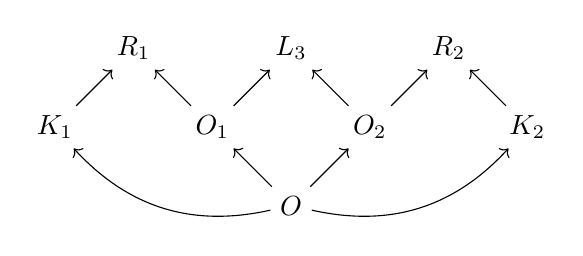
\begin{tikzpicture} %[scale=0.8]
      \node (o) at (0,-1) {\(O\)};
      \node (r3) at (0,1) {\(L_3\)};
      \node (o1) at (-1,0) {\(O_1\)};
      \node (o2) at (1,0) {\(O_2\)};
      \node (r1) at (-2,1) {\(R_1\)};
      \node (r2) at (2,1) {\(R_2\)};
      \node (k1) at (-3,0) {\(K_1\)};
      \node (k2) at (3,0) {\(K_2\)};
      \draw [->] (o) -- (o1);
      \draw [->] (o) -- (o2);
      \draw [->] (o1) -- (r3);
      \draw [->] (o2) -- (r3);
      \draw [->] (o1) -- (r1);
      \draw [->] (o2) -- (r2);
      \draw [->] (k1) -- (r1);
      \draw [->] (k2) -- (r2);
      \draw [->] (o) to [bend left] (k1);
      \draw [->] (o) to [bend right] (k2);
    \end{tikzpicture}
    \]
    Moreover
    \begin{align*}
      t_1^{-1}\dashv t_2^{-1}\implies\text{ there exists the morphisms }O\emb K_1\text{ and }\\
      t_2^{-1}\dashv t_1^{-1}\implies\text{ there exists the morphisms }O\emb K_2.
    \end{align*}
  \item
    \label{lem:constraint_join}
    If $t_3 <_{\theta} t_1$ and $t_3<_{\theta} t_2$, then let $O_1$, $O_2$ be two graphs such that the causal pairs of $t_3 <_{\theta} t_1$ and $t_3<_{\theta} t_2$ are induced by $O_1$ and $O_2$ respectively.
Let $O_1\remb O\lemb O_2$ be the pullback of the span $O_1\lemb R_3 \remb O_2$. If $t_1\not\dashv t_2$ and $t_2\not\dashv t_1$
then there exists the morphisms $O\emb K_1$ and $O\emb K_2$ such that the diagram below commutes:
    \[
    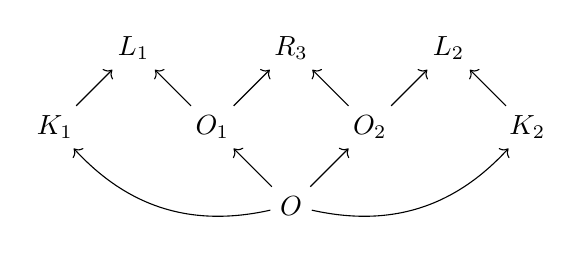
\begin{tikzpicture} %[scale=0.8]
      \node (o) at (0,-1) {\(O\)};
      \node (r3) at (0,1) {\(R_3\)};
      \node (o1) at (-1,0) {\(O_1\)};
      \node (o2) at (1,0) {\(O_2\)};
      \node (r1) at (-2,1) {\(L_1\)};
      \node (r2) at (2,1) {\(L_2\)};
      \node (k1) at (-3,0) {\(K_1\)};
      \node (k2) at (3,0) {\(K_2\)};
      \draw [->] (o) -- (o1);
      \draw [->] (o) -- (o2);
      \draw [->] (o1) -- (r3);
      \draw [->] (o2) -- (r3);
      \draw [->] (o1) -- (r1);
      \draw [->] (o2) -- (r2);
      \draw [->] (k1) -- (r1);
      \draw [->] (k2) -- (r2);
      \draw [->] (o) to [bend left] (k1);
      \draw [->] (o) to [bend right] (k2);
    \end{tikzpicture}
    \]
    Moreover
    \begin{align*}
      t_1\dashv t_2\implies\text{ there exists the morphisms }O\emb K_1\text{ and }\\
      t_2\dashv t_1\implies\text{ there exists the morphisms }O\emb K_2.
    \end{align*}
  \end{enumerate}
\end{lemma}
\begin{proof}
  \begin{enumerate}
  \item
    %% If $\theta$ is a causal trace then we can show that there exists $t_1'$ and $t_2'$ such that $t_1\congr t_1'$, $t_2\congr t_2'$ and such that the transitions $t_1';t_2';t_3$ are composable and such that $t_1'\Diamond_{\text{seq}} t_2'$.
    %% %
    %% Let $\theta'$ be the smallest subtrace of $\theta$ that contains all three transitions $t_1$, $t_2$ and $t_3$. Suppose that $t_1$ occurs before $t_2$, that is $\theta':t_1;\cdots t_2\cdots t_3$.
    %% From $t_2<_{\theta} t_3$ we have that there exists $t_2'$ such that $t_2'< t_3$. It implies that there exists a trace $\theta_1\congr\theta'$ such that $t_2';t_3$ is at the end of $\theta'$.
    %% Using a similar argument as above, there exist $t_1'$ such that $t_1'<_{\theta} t_3$ and we can rewrite $\theta$ to $\theta_1$ ending in $t_1';t_2';t_3$ and with $t_1'\Diamond_{\text{seq}} t_2'$.
    %% %
    %% Consider now the trace $t_1';t_2';t_3$ with $t_2':M_2\remb D_2 \lemb M_3$. We can rewrite $t_1';t_2';t_3$ as $t_2'';t_1'';t_3$, with $t_1'\congr t_1''$ and $t_2'\congr t_2''$. Then we also have the trace $t_2';t_1''^{-1}$ with the two transition sequential independent. Therefore we have that there exists a morphism $R_1\emb D_2$ that makes the diagram commute.

    From $t_1<_{\theta} t_3$ we have that there exists $t_1'\simeq t_1$ such that $t_1';t_3$. Let us denote
$t_1':M_1\remb D_1 \lemb M_3$ the transition $t_1'$. Similarly, from $t_2<_{\theta} t_3$ there exists $t_2\simeq t_2$, $t_2';t_3$ and $t_2':M_2\remb D_2 \lemb M_3$.
    We can show that there exists a morphism $R_1\to D_2$ such that the diagram below commutes iff there is also a morphism $O\to K_2$ that commutes.
    \[
    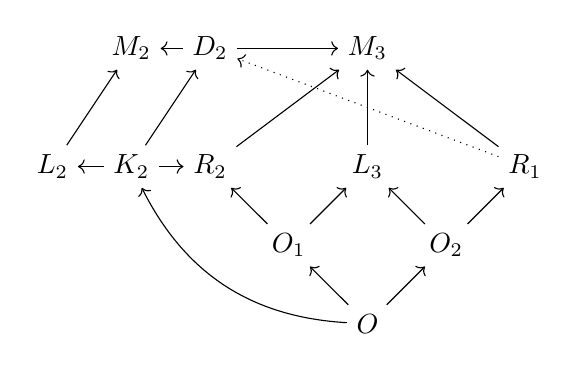
\begin{tikzpicture} %[scale=0.8]
      \node (o) at (0,-1) {\(O\)};
      \node (r3) at (0,1) {\(L_3\)};
      \node (o1) at (-1,0) {\(O_1\)};
      \node (o2) at (1,0) {\(O_2\)};
      \node (r1) at (-2,1) {\(R_2\)};
      \node (r2) at (2,1) {\(R_1\)};
      \node (k1) at (-3,1) {\(K_2\)};
      \node (l1) at (-4,1) {\(L_2\)};
      \node (m3) at (0,2.5) {\(M_3\)};
      \node (d2) at (-2,2.5) {\(D_2\)};
      \node (m2) at (-3,2.5) {\(M_2\)};
      \draw [->] (o) -- (o1);
      \draw [->] (o) -- (o2);
      \draw [->] (o1) -- (r3);
      \draw [->] (o2) -- (r3);
      \draw [->] (o1) -- (r1);
      \draw [->] (o2) -- (r2);
      \draw [->] (k1) -- (r1);
      \draw [->] (o) to [bend left] (k1);
      \draw [->] (k1) -- (l1);
      \draw [->] (d2) -- (m2);
      \draw [->] (d2) -- (m3);
      \draw [->] (k1) -- (d2);
      \draw [->] (l1) -- (m2);
      \draw [->] (r1) -- (m3);
      \draw [->] (r3) -- (m3);
      \draw [->] (r2) -- (m3);
      \draw [dotted,->] (r2) -- (d2);
    \end{tikzpicture}
    \]
    We have then that if $t_2\not\dashv t_1$ then the morphism $O\to K_2$ above exists and moreover if there is no morphism $O\to K_2$ that commutes then $t_2\dashv t_1$. We reason similarly for $t_1\dashv t_2$.

    From~\autoref{lem:inhibiting_pair}, if $t_2\dashv t_1$ then $t_1\not\dashv t_2$ and hence there exists $O\to K_1$ that commutes.
    \item The proof is similar to the one above.
  \end{enumerate}
\end{proof}

Inutuitively,~\autoref{lem:constraint_mj} says that if two events cannot \emph{produce} the same resource (\autoref{lem:constraint_meet}) and the same resource cannot be \emph{consumed} twice (\autoref{lem:constraint_join}). Let us give some examples.
\begin{example}
  For the following rules:
  \[
  r_1:\varepsilon \Rightarrow A,B \qquad r_2: \varepsilon \Rightarrow A,C \qquad r_3: A,B,C \Rightarrow D
  \]
  there is a trace where $t_1<t_3$ and $t_2<t_3$, however both cannot produce $A$:
    \[
    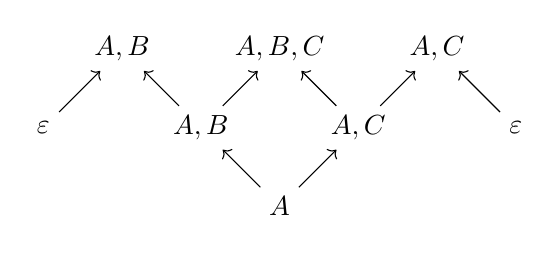
\begin{tikzpicture} %[scale=0.8]
      \node (o) at (0,-1) {\(A\)};
      \node (r3) at (0,1) {\(A,B,C\)};
      \node (o1) at (-1,0) {\(A,B\)};
      \node (o2) at (1,0) {\(A,C\)};
      \node (r1) at (-2,1) {\(A,B\)};
      \node (r2) at (2,1) {\(A,C\)};
      \node (k1) at (-3,0) {\(\varepsilon\)};
      \node (k2) at (3,0) {\(\varepsilon\)};
      \draw [->] (o) -- (o1);
      \draw [->] (o) -- (o2);
      \draw [->] (o1) -- (r3);
      \draw [->] (o2) -- (r3);
      \draw [->] (o1) -- (r1);
      \draw [->] (o2) -- (r2);
      \draw [->] (k1) -- (r1);
      \draw [->] (k2) -- (r2);
    \end{tikzpicture}
    \]
  %% \[
  %% t_1: A \Rightarrow A,B \qquad t_2: A \Rightarrow A,C \qquad t_3: A,B,C \Rightarrow D
  %% \]
  %% we can indeed have that both $t_1<t_3$ and $t_2<t_3$.
\end{example}
\begin{example}
  Consider the transitions
  \[
  t_3: \varepsilon \Rightarrow A\qquad t_1: A\Rightarrow \varepsilon \qquad t_2: A\Rightarrow \varepsilon
  \]
  for which there is no trace where both $t_3<t_1$ and $t_3<t_2$ hold. The resource $A$ produced by $t_1$ can only be consumed once.
  If, however, $t_1$ and $t_2$ do not consume $A$ but preserve it:
  \[
  t_3: \varepsilon \Rightarrow A\qquad t_1: A\Rightarrow A,B \qquad t_2: A\Rightarrow A,C
  \]
  then indeed both $t_1<t_3$ and $t_2<t_3$ hold.
\end{example}
  %% Note that though the following trace $\theta$, produced by transitions $t_3;t_1;t_2$, is valid
  %% \[
  %% \theta:\varepsilon \Rightarrow A \Rightarrow A, B\Rightarrow B\qquad t_3: \varepsilon \Rightarrow A\qquad t_1: A\Rightarrow A,B\qquad t_2: A\Rightarrow \varepsilon
  %% \]
  %% we cannot deduce $t_3<t_2'$, for $t_2'\congr t_2$, as in the trace $\theta$ above, transitions cannot commute.
\begin{example}
  For a trace $t_1;t_2;t_3$ with the transitions
  \[
  t_1: A \Rightarrow A,B\qquad t_2: A,B\Rightarrow B,C \qquad t_3: B,C\Rightarrow D
  \]
  one cannot deduce $t_1<t_3$, as transitions $t_1$ and $t_2$ do not commute.
\end{example}


%% \begin{remark}
%%   Sequential dependence (~\autoref{def:seq_dep}) is not transitive. Therefore when considering posets in~\autoref{def:poset}, we need to distinguish between the \emph{immediate} order relation (the cover relation in~\autoref{def:poset}) and its transitive closure. %We denote the first $\cover$ and the latter with $\tleq$.
%% \end{remark}

\begin{lemma}
  \label{lem:constraint_inhibit}
  Let $\theta$ a causal trace and let $t_1:M_1\overset{m_1,p_1}{\Rightarrow}N_1$ and $t_2:M_2\overset{m_2,p_2}{\Rightarrow}N_2$ be two transitions in $\theta$.
  If $t_1 \leq t_2$ then $t_2\not\dashv t_1$.
\end{lemma}
\begin{proof}[Proof sketch]
  One cannot commute $t_1$ and $t_2$ such that $t_1':M\overset{m_1,p_1}{\Rightarrow}N_1$ and $t_2':M\overset{m_2,p_2}{\Rightarrow}N_2$, for some $t_1'\simeq t_1$, $t_2'\simeq t_2$. Therefore one cannot deduce that the pair are not parallel independent.
\end{proof}

\begin{definition}[Augmented poset]
  Let $s=(E,\cover,\dashv,\labl)$ be a set of events equipped with two binary relations on events $\cover$ and $\dashv$ and a labelling function $\labl:E\to R$. We can retrive a poset from $s$, denoted $(E,\leq)$, where $\leq$ is the transitive and reflexive closure of $\cover$.
  %Let $s=(E, \leq,\dashv,\labl)$ be a set of events equipped with a partial order $\leq$, a binary relation on events $\dashv$ and a labelling function $\labl:E\to R$.
  We call $s$ an \emph{augmented poset}.
\end{definition}

\begin{definition}[Decorated poset]
  \begin{enumerate}
  \item[] $~$
  \item Given a set of events $E$ and a labeling function $\labl$ on events, define a function $\decor:E\times E \to E\times E\times G$ that associates to a pair of events $(e,e')$ the following set
    \begin{align*}
      \decor_{+}(e,e') = \{(e,e',O) : O\text{ is a graph such that }\labl(e)\redl{+}_O \labl(e')\}\\
       \decor_{-}(e,e') = \{(e,e',O) : O\text{ is a graph such that }\labl(e)\redl{-}_O \labl(e')\}
    \end{align*}

  \item Let $s = (E,\cover,\dashv,\labl)$ be an augmented poset. A \emph{decorated} poset of $s$, denoted $s^{\star}$, is defined as follows
    \begin{align*}
      s^{\star} = (E,\redl{+},\redl{-},\labl), \text{ where }
      &e\redl{+}_O e' \iff (e,e',O)\in\decor_+(e,e')\text{ and }e\cover e'\\
      &e\redl{-}_O e' \iff (e,e',O)\in\decor_-(e,e')\text{ and }e\dashv e'\\
    \end{align*}
    We denote $\decor(s)$ the set of all decorated posets of $s$.
  \end{enumerate}
\end{definition}

Note that the notation $e\redl{+}_O e'$ is an overload of the notation $\labl(e)\redl{+}_O \labl(e')$. The first is defined on events using the abstraction function. The second, defined on rules, can be inferred from the rules itself.

\begin{definition}[The abstraction on a trace]
  \label{def:abstraction}
  Let us denote with $\Theta$ the set of causal traces.
  Define $\alpha:\Theta\to\mathcal{S}$ an \emph{abstraction} function that maps a trace into a poset as follows:
    \begin{itemize}
    \item given a transition $t:M\overset{m,p}{\Rightarrow} M'$ define the \emph{abstract event} $e$ associated to it
      $\alpha(t) = e_t$ such that $\labl(e) = p$.
    %% \item define an augmented poset from a trace $\alpha(\theta) = (E,\cover,\dashv,\labl)$ such that $\alpha$ is a bijection between transitions and abstract events and such that the sequential dependence and inhibition relations between transitions is preserved:
    %%   \begin{align*}
    %%     %\alpha(t_i:M_{i-1}\overset{m_{i},p_{i}}{\Rightarrow}M_i) = e_i \\
    %%     e_i \cover e_j \iff t_i <_{\theta} t_j \text{ and } \alpha(t_i)=e_i, \alpha(t_j)=e_j\\
    %%     e_i \dashv e_j \iff t_i \dashv_{\theta} t_j \text{ and } \alpha(t_i)=e_i, \alpha(t_j)=e_j.
    %%   \end{align*}
    \item define a decorated poset from a trace $\alpha(\theta) = (E,\redl{+},\redl{-},\labl)$ such that $\alpha$ is a bijection between transitions and abstract events and such that the sequential dependence and inhibition relations between transitions is preserved:
      \begin{align*}
        %\alpha(t_i:M_{i-1}\overset{m_{i},p_{i}}{\Rightarrow}M_i) = e_i \\
        e_i \redl{+}_O e_j \iff t_i <_{\theta} t_j, \labl(t_i) \redl{+}_O \labl(t_j)
        \text{ and } \alpha(t_i)=e_i, \alpha(t_j)=e_j\\
        e_i \redl{-}_O e_j \iff t_i \dashv_{\theta} t_j, \labl(t_i) \redl{-}_O \labl(t_j)
        \text{ and } \alpha(t_i)=e_i, \alpha(t_j)=e_j.
      \end{align*}
    \end{itemize}
  %\item
    Let $\Theta = \{\theta_1,\cdots,\theta_n\}$ be a set of causal traces.
    Define the set of decorated posets $\mathcal{S}$ obtained by abstraction on $\Theta$ as follows
    \[
    \alpha(\{\theta_1,\cdots,\theta_n\}) = (s_1,\cdots, s_k)\text{ with }k\leq n
    \]
    where for each decorated poset $s$ there exists at least one trace $\theta\in\Theta$ such that $\alpha(\theta) = s$.
  %\end{itemize}
\end{definition}

\begin{definition}[Valid decorated poset]
  \label{def:constraints_poset}
  A decorated poset $s = (E,\redl{+},\redl{-},\labl)$ is \emph{valid} if the following hold:
  \begin{description}
  \item[directed]
    $s$ is directed w.r.t. the transitive and reflexive closure of $\redl{+}$;
  \item[events are not pairwise inhibiting]
    $\forall e_1,e_2\in s$, $e_1\redl{-}_s e_2\implies \neg(e_2 \redl{-}_{s'} e_1)$, for some $s$, $s'$;
  \item[events cannot inhibit their causes]
    $\forall e_1,e_2\in s$, $e_1\leq e_2\implies \neg(e_2 \redl{-}_{s} e_1)$, for some $s$;
  \item[constraints on decorating meets]
    $\forall e_1,e_2,e_3\in s$ such that $e_1\redl{+}_{s_1} e_3$ and $e_2\redl{+}_{O_2} e_3$, let $O_1\remb O\lemb O_2$ be the pullback of the span $O_1\lemb L_3 \remb O_2$.
If there is no $s$, $s'$ such that $e_1\redl{-}_s e_2$ and $e_2\redl{-}_{s'} e_1$ then there exists the morphisms $O\emb K_1$ and $O\emb K_2$ such that the diagram below commutes:
    \[
    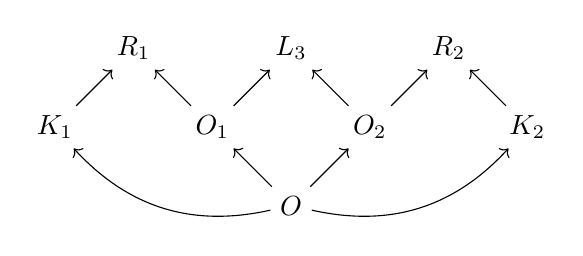
\begin{tikzpicture} %[scale=0.8]
      \node (o) at (0,-1) {\(O\)};
      \node (r3) at (0,1) {\(L_3\)};
      \node (o1) at (-1,0) {\(O_1\)};
      \node (o2) at (1,0) {\(O_2\)};
      \node (r1) at (-2,1) {\(R_1\)};
      \node (r2) at (2,1) {\(R_2\)};
      \node (k1) at (-3,0) {\(K_1\)};
      \node (k2) at (3,0) {\(K_2\)};
      \draw [->] (o) -- (o1);
      \draw [->] (o) -- (o2);
      \draw [->] (o1) -- (r3);
      \draw [->] (o2) -- (r3);
      \draw [->] (o1) -- (r1);
      \draw [->] (o2) -- (r2);
      \draw [->] (k1) -- (r1);
      \draw [->] (k2) -- (r2);
      \draw [->] (o) to [bend left] (k1);
      \draw [->] (o) to [bend right] (k2);
    \end{tikzpicture}
    \]
  \item[constraints on decorating joins]
    $\forall e_1,e_2,e_3\in s$ such that $e_3\redl{+}_{s_1} e_1$ and $e_3\redl{+}_{O_2} e_2$, let $O_1\remb O\lemb O_2$ be the pullback of the span $O_1\lemb L_3 \remb O_2$.
    If there is no $s$, $s'$ such that $e_1\redl{-}_s e_2$ and $e_2\redl{-}_{s'} e_1$ then there exists the morphisms $O\emb K_1$ and $O\emb K_2$ such that the diagram below commutes:
       \[
    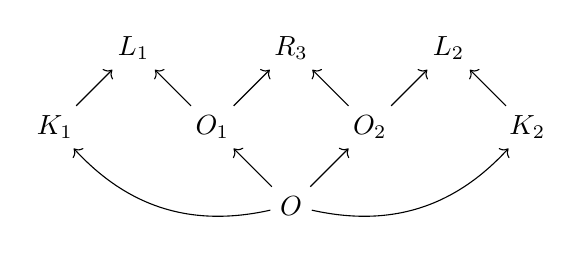
\begin{tikzpicture} %[scale=0.8]
      \node (o) at (0,-1) {\(O\)};
      \node (r3) at (0,1) {\(R_3\)};
      \node (o1) at (-1,0) {\(O_1\)};
      \node (o2) at (1,0) {\(O_2\)};
      \node (r1) at (-2,1) {\(L_1\)};
      \node (r2) at (2,1) {\(L_2\)};
      \node (k1) at (-3,0) {\(K_1\)};
      \node (k2) at (3,0) {\(K_2\)};
      \draw [->] (o) -- (o1);
      \draw [->] (o) -- (o2);
      \draw [->] (o1) -- (r3);
      \draw [->] (o2) -- (r3);
      \draw [->] (o1) -- (r1);
      \draw [->] (o2) -- (r2);
      \draw [->] (k1) -- (r1);
      \draw [->] (k2) -- (r2);
      \draw [->] (o) to [bend left] (k1);
      \draw [->] (o) to [bend right] (k2);
    \end{tikzpicture}
    \]
  \end{description}
  where $\labl(e_i)=r_i:L_i\remb K_i\lemb R_i$.
\end{definition}

\begin{lemma}
  \label{prop:constraints_poset}
  For any causal trace $\theta$, $\alpha(\theta)$ is a valid decorated poset.
\end{lemma}
\begin{proof}
  It is straigthforward from~\autoref{def:causal_trace},~\autoref{lem:inhibiting_pair},~\autoref{lem:constraint_inhibit} and \autoref{lem:constraint_mj}.
\end{proof}

If we work only on augmented posets, the abstraction is "too forgetful".
The following examples give an intuition of why the abstraction function has to preserve the inhibition relation and the decorations on causality and inhibition.
We make this intuition formal in~\autoref{th:correction}.

\begin{example}
  Let us consider the following rules and trace:
  \begin{align*}
    r_1:A \Rightarrow A, B\qquad r_2:A \Rightarrow C \qquad r_3: B,C \Rightarrow C\qquad
    A \overset{\id_A,r_1}{\Rightarrow} A, B \overset{\id_A,r_2}{\Rightarrow} B,C \overset{id_{B,C},r_3}{\Rightarrow}C.
  \end{align*}
  Let us denote $t_1$, $t_2$ and $t_3$ the three transitions. We have that $t_1<t_3$, $t_2<t_3$ and $t_2\dashv t_1$. If we "forget" that $t_2\dashv t_1$ we retrieve a trace where $t_1$ and $t_2$ are sequential independent:
  \begin{align*}
    A_1,A_2 \overset{\id_{A_1},r_1}{\Rightarrow} A_1,A_2,B \overset{\id_{A_2},r_2}{\Rightarrow} A_1,B,C \overset{id_{B,C},r_3}{\Rightarrow} A_1,C.
  \end{align*}
  From such an abstraction it is not possible to recover the original trace.
\end{example}

%% \begin{example} - for the cover relation
%%   Let us consider the following rules:
%%   \begin{align*}
%%     r_1:\varepsilon \Rightarrow A, B\qquad r_2:A \Rightarrow C \qquad r_3: B,C \Rightarrow C
%%   \end{align*}
%%   and the trace
%%   \begin{align*}
%%     \varepsilon \overset{\emptyset,r_1}{\Rightarrow} A, B \overset{\id_A,r_2}{\Rightarrow} B,C \overset{id_{B,C},r_3}{\Rightarrow}C.
%%   \end{align*}
%%   Let us denote $t_1$, $t_2$ and $t_3$ the three transitions. We have that $t_1<t_3$, $t_2<t_3$ and $t_1< t_2$. If we "forget" that $t_1< t_3$ (as both $t_1<t_2$ and $t_2<t_3$ hold), we retrieve the following trace:
%%   \begin{align*}
%%     B_1 \overset{\emptyset,r_1}{\Rightarrow} B_1,A,B_2 \overset{\id_{A},r_2}{\Rightarrow} B_1,A,B_2,C \overset{id_{B_1,C},r_3}{\Rightarrow} B_2,A_1,C.
%%   \end{align*}
%% \end{example}

\begin{example}
  If, in the following trace $\theta$, produced by the transitions $t_1;t_2;t_3$, we forget the decoration we obtain a poset with three events $e_1,e_2,e_3$ such that $e_1<e_3$ and $e_2<e_3$.
  \[
  \theta:\varepsilon \Rightarrow A \Rightarrow A,B\Rightarrow A,B,C\qquad t_1: \varepsilon \Rightarrow A\qquad t_2: \varepsilon\Rightarrow A,B\qquad t_2: A,B\Rightarrow A,B,C
  \]
  But we can come up with two decorations for such poset, where one of them leads to a invalid decorated poset:
  \begin{align*}
  \text{good decoration: }&e_1\redl{+}_A e_3\qquad e_2\redl{+}_B e_3\\
  \text{bad decoration: }&e_1\redl{+}_A e_3\qquad e_2\redl{+}_A e_3
  \end{align*}
\end{example}

\subsection{Interpreting inhibition on posets}

%In interpreting our logic, we work with a set of posets in $\mathcal{S}$ and a set of events $\cup_{s\in\mathcal{S}} E_s$.

\begin{definition}[Linear extensions of posets]
  A linear extension, denoted $\underline{s}$, of a poset $s=(E,\tleq)$ is any total order that extends the partial order $\tleq$. We denote $\linear(s)$ the set of all possible linear extensions of $s$.
  %% \[
  %% (E,\seq)\in\linear(s) \iff \forall e_1,e_2\in E, e_1\leq e_2\implies e_1\seq e_2.
  %% \]
  A linear extension of a augmented poset $s=(E,\cover,\dashv)$ is any total order such that
  \begin{align*}
    (E,\seq)\in\linear(s) \iff \forall e_1,e_2\in E, &e_1\leq e_2\implies e_1\seq e_2\\
    & e_1\dashv e_2\implies e_2\seq e_1.
  \end{align*}
\end{definition}

\begin{definition}
  Let $\underline s=(E,\seq\redl{+},\redl{-},\labl)$ be a linear extension of a decorated poset $s$. A \emph{concretisation} function  $\mathtt{Concret}:E\leftrightarrow \{t_1,\cdots t_n\}$ is a bijection between events in $E$ and a set of transitions such that
  \begin{align*}
    e_1\redl{+}_s e_2 \iff& \mathtt{Concret}(e_1) = t_1, \mathtt{Concret}(e_1) = t_2, \text{ such that }t_1<_{t_1;t_2}t_2\\
    &\text{ and the causal pair of }t_1<_{t_1;t_2}t_2\text{ is induced by }s.
  \end{align*}
\end{definition}


\begin{definition}[Refinement of an event in a poset]
  Let $e$ be an event in a decorated poset $s=(E,\redl{+},\redl{-},\labl)$.
  Define $\mathtt{Concret}(e\in s) = \mathtt{Concret}(e)$ for $\mathtt{Concret}:\underline{s}\to\{t_1,\cdots t_n\}$ a concretisation function.
  %We call such a graph $M$ a \emph{context of application} of $e$ in $s$.
\end{definition}

\begin{definition}[Refinement based on negative influence]
\label{def:ref_neg_infl}
  For two posets $s_1,s_2$ and two events $e_1\in s_1$ and $e_2\in s_2$ such that  $\mathtt{Concret}(e_1\in s_1) = M_1\Rightarrow N_1$ and $\mathtt{Concret}(e_2\in s_2) = M_2\Rightarrow N_2$, define $\mathtt{Concret}(e_1\in s_1\redl{-} e_2\in s_2) = M$ for which the diagram below commutes:
  \[
  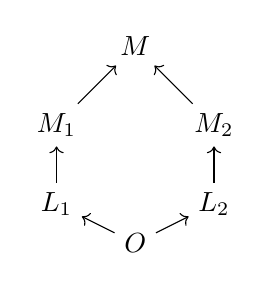
\begin{tikzpicture} %[scale=0.8]
    \node (o) at (0,-0.5) {\(O\)};
    \node (n) at (0,2) {\(M\)};
    \node (l1) at (-1,0) {\(L_1\)};
    \node (l2) at (1,0) {\(L_2\)};
    \node (n1) at (-1,1) {\(M_1\)};
    \node (n2) at (1,1) {\(M_2\)};
    \draw [->] (l1) -- (n1);
    \draw [->] (l2) -- (n2);
    \draw [->] (o) -- (l1);
    \draw [->] (o) -- (l2);
    \draw [->] (n1) -- (n);
    \draw [->] (n2) -- (n);
  \end{tikzpicture}
  \]
  where $\labl(e_1)\redl{-}_s\labl(e_2)$, for some cospan $s:L_1\remb O\lemb L_2$.
\end{definition}

\subsection{From posets to traces}
%
\begin{lemma}
  Let $\theta:M_2\Rightarrow M_3\cdots M_n\Rightarrow M_{n+1}$ be a trace and let $t_1:M_1\Rightarrow M_n$ be a transition. Let $\alpha(\theta,t_1) = (E,\sqsubset,\labl)$ be its abstraction such that the following hold:
  \begin{enumerate}
  \item $\forall i, 2\leq i\leq n$, $e_1\sqsubset_{O_1} e_i\iff e_i = e_n$;
  \item $(E,\sqsubset,\labl)$ is a valid decoration, according to~\autoref{def:constr_dec};
  \end{enumerate}
Then we can rewrite $\theta$ into $\theta':M_1'\Rightarrow M_2\Rightarrow M_3\cdots M_n\Rightarrow M_{n+1}$ for which $\alpha(\theta)\iso\alpha(\theta')$ and the conditions above hold.
\end{lemma}
\begin{proof}
  We proceed by induction on the trace $M_2\Rightarrow M_3\cdots M_j\Rightarrow M_{j+1}\cdots M_n\Rightarrow M_{n+1}$.

  First we introduce some notations we will need during the proof. Let us denote $\prec$ the ordering between transitions in $\theta$.
  For an event $e_j$ we say that an event $e_i$ is a $\sqsubset$-$\prec$-successor, if it is a succesor for the $\sqsubset$ relation and the latest one in the $\prec$ ordering (that is for transitions $t_i$ and $t_j$ such that $\alpha(t_i)=e_i$, $\alpha(t_j)=e_j$ we have that $t_i\prec t_j$).
  For a transition $t_i:M_i{\Rightarrow} M_{i+1}$, if $\alpha(t_i)=e_i$, then we write $M_i\overset{e_i}{\Rightarrow} M_{i+1}$.

  Let us consider one step of swapping: let $t_j:M_j\overset{e_j}{\Rightarrow} M_{j+1}$ and $t_1^j:P_j\overset{e_1}{\Rightarrow}M_{j+1}$ where $2\leq j\leq n-1$. %and $\alpha(t_j)=e_j$, $\alpha(t_1^j) = e_1$.
  \[
  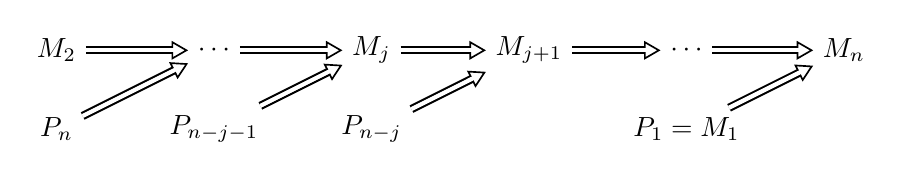
\begin{tikzpicture} %[scale=0.8]
    \node (m2) at (0,1) {\(M_2\)};
    \node (dots) at (2,1) {\(\cdots\)};
    \node (mj) at (4,1) {\(M_j\)};
    \node (mj1) at (6,1) {\(M_{j+1}\)};
    \node (dots2) at (8,1) {\(\cdots\)};
    \node (mk) at (10,1) {\(M_n\)};
    \node (pk) at (0,0) {\(P_n\)};
    \node (pkj1) at (2,0) {\(P_{n-j-1}\)};
    \node (pkj) at (4,0) {\(P_{n-j}\)};
    \node (p1) at (8,0) {\(P_{1}=M_1\)};
    \draw [vecArrow] (m2) -- (dots);
    \draw [vecArrow] (dots) -- (mj);
    \draw [vecArrow] (mj) -- (mj1);
    \draw [vecArrow] (mj1) -- (dots2);
    \draw [vecArrow] (dots2) -- (mk);
    \draw [vecArrow] (pk) -- (dots);
    \draw [vecArrow] (pkj1) -- (mj);
    \draw [vecArrow] (pkj) -- (mj1);
    \draw [vecArrow] (p1) -- (mk);
  \end{tikzpicture}
  \]
  We can rewrite the transitions $M_j\overset{e_j}{\Rightarrow} M_{j+1}\overset{e_1^{-1}}{\Rightarrow} P_{n-j}$, as productions are reversible. We distinguish between two cases. In the diagram below:
    \[
    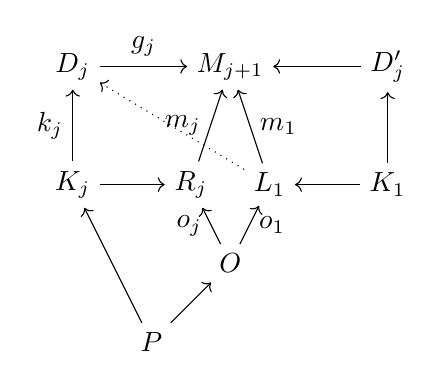
\begin{tikzpicture} %[scale=0.8]
    \node (r1) at (1.5,0) {\(R_j\)};
    \node (m1) at (2,1.5) {\(M_{j+1}\)};
    \node (l2) at (2.5,0) {\(L_1\)};
    \node (d1) at (0,1.5) {\(D_j\)};
    \node (k1) at (0,0) {\(K_j\)};
    \node (d2) at (4,1.5) {\(D_j'\)};
    \node (k2) at (4,0) {\(K_1\)};
    \node (o) at (2,-1) {\(O\)};
    \node (p) at (1,-2) {\(P\)};
    \draw [->] (k1) -- (r1);
    \draw [->] (k2) -- (l2);
    \draw [->] (k1) -- node [left,midway] {\(k_j\)} (d1);
    \draw [->] (k2) -- (d2);
    \draw [->] (d1) -- node [above,midway] {\(g_j\)} (m1);
    \draw [->] (d2) -- (m1);
    \draw [->] (l2) -- node [right,midway] {\(m_1\)} (m1);
    \draw [->] (r1) -- node [left,midway] {\(m_j\)} (m1);
    \draw [dotted,->] (l2) -- (d1);
    \draw [->] (p) -- (k1);
    \draw [->] (p) -- (o);
    \draw [->] (o) -- node [left,midway] {$o_j$} (r1);
    \draw [->] (o) -- node [right,midway] {$o_1$} (l2);
    \end{tikzpicture}
    \]
    first suppose that there is a morphism $R_1\to D_j$ such that the diagram commutes. Then we can rewrite $M_j$ using the production of $e_1^{-1}$ and obtain the transition $M_j\overset{e_1^{-1}}{\Rightarrow}P_{j+1}$. We reverse it again and obtain $P_{j+1}\overset{e_1}{\Rightarrow} M_j$. Then the induction continues with the transitions $M_{j-1}\overset{e_{j-1}}{\Rightarrow} M_{j}$ and $P_{j+1}\overset{e_1}{\Rightarrow} M_j$.

    The second case is when there is no such morphism.
    We consider the following cases:

    \begin{itemize}
    \item {\bf both events have a common $\sqsubset$-$\prec$-successor}. Note that from the first condition in the hypothesis, this case is only possible if $e_j\sqsubset e_n$. As $e_n$ is the $\sqsubset$-$\prec$-successor of $e_j$ we have that for all events $e_i$ such that $\alpha(t_i)=e_i$ and $j<i<k$, $e_j$ and $e_i$ are sequential independent.
      \begin{mdframed}[backgroundcolor=blue!20]
        not if we consider inhibition!
      \end{mdframed}
      Therefore can rewrite the trace $M_j{\Rightarrow} M_{j+1}\cdots M_n\Rightarrow M_{n+1}$ such that $M_j'\overset{e_j}{\Rightarrow}M_n\overset{e_n}{\Rightarrow}M_{n+1}$.
      The diagram above becomes then
    \[
    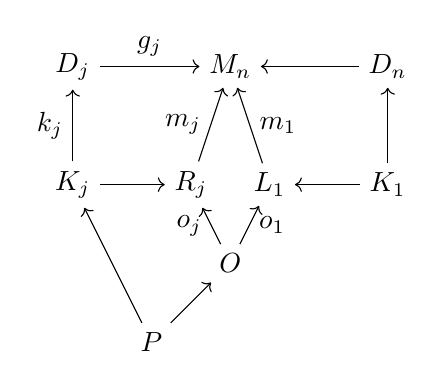
\begin{tikzpicture} %[scale=0.8]
    \node (r1) at (1.5,0) {\(R_j\)};
    \node (m1) at (2,1.5) {\(M_{n}\)};
    \node (l2) at (2.5,0) {\(L_1\)};
    \node (d1) at (0,1.5) {\(D_j\)};
    \node (k1) at (0,0) {\(K_j\)};
    \node (d2) at (4,1.5) {\(D_n\)};
    \node (k2) at (4,0) {\(K_1\)};
    \node (o) at (2,-1) {\(O\)};
    \node (p) at (1,-2) {\(P\)};
    \draw [->] (k1) -- (r1);
    \draw [->] (k2) -- (l2);
    \draw [->] (k1) -- node [left,midway] {\(k_j\)} (d1);
    \draw [->] (k2) -- (d2);
    \draw [->] (d1) -- node [above,midway] {\(g_j\)} (m1);
    \draw [->] (d2) -- (m1);
    \draw [->] (l2) -- node [right,midway] {\(m_1\)} (m1);
    \draw [->] (r1) -- node [left,midway] {\(m_j\)} (m1);
    \draw [->] (p) -- (k1);
    \draw [->] (p) -- (o);
    \draw [->] (o) -- node [left,midway] {$o_j$} (r1);
    \draw [->] (o) -- node [right,midway] {$o_1$} (l2);
    \end{tikzpicture}
    \]

    We have that for the transitions $M_j'\overset{e_j}{\Rightarrow}M_n\overset{e_n}{\Rightarrow}M_{n+1}$ that the underlying positive influence is $e_j\redl{+}_{O_j} e_n$ and similarly for $e_1\redl{+}_{O_1}e_n$. We obtain the following diagram
    \[
    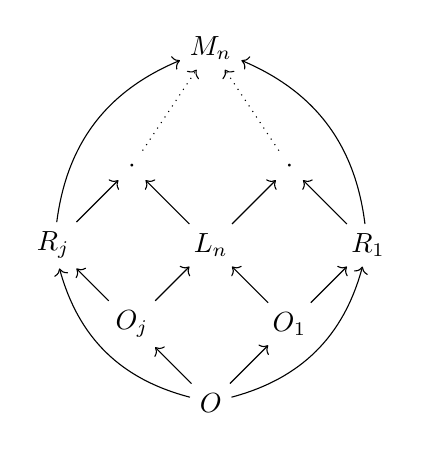
\begin{tikzpicture} %[scale=0.8]
    \node (mn) at (0,2.5) {\(M_{n}\)};
    \node (ln) at (0,0) {\(L_{n}\)};
    \node (o) at (0,-2) {\(O\)};
    \node (oj) at (-1,-1) {\(O_j\)};
    \node (o1) at (1,-1) {\(O_1\)};
    \node (rj) at (-2,0) {\(R_j\)};
    \node (r1) at (2,0) {\(R_1\)};
    \node (d1) at (-1,1) {\(\cdot\)};
    \node (d2) at (1,1) {\(\cdot\)};
    \draw [->] (o) -- (o1);
    \draw [->] (o) -- (oj);
    \draw [->] (oj) -- (rj);
    \draw [->] (oj) -- (ln);
    \draw [->] (o1) -- (r1);
    \draw [->] (o1) -- (ln);
    \draw [->] (rj) -- (d1);
    \draw [->] (ln) -- (d1);
    \draw [->] (r1) -- (d2);
    \draw [->] (ln) -- (d2);
    \draw [dotted,->] (d1) -- (mn);
    \draw [dotted,->] (d2) -- (mn);
    \draw [->] (o) to [bend right] (r1);
    \draw [->] (o) to [bend left] (rj);
    \draw [->] (r1) to [bend right] (mn);
    \draw [->] (rj) to [bend left] (mn);
    \end{tikzpicture}
    \]
    where $O\emb O_j$ and $O\emb O_1$. This contradicts the constraints of~\autoref{def:constr_dec}.


    \item {\bf events have different $\sqsubset$-$\prec$-successors}. Let $e_i$ be the succesor of $e_j$, $e_j\sqsubset e_i$ with $i\neq k$.
      We will show that this case is not possible. %To do this we have to reason by induction on the trace

      If there is no morphism $j$ then there exists $O$ the pullback of $R_j\lemb M_{j+1}\remb L_1$ and $P$ the pullback of $K_j\lemb R_j\remb O$ such that the morphism $P\to O$ is not an iso.

    Let us suppose that
    \begin{align}
      \label{eq:ekei}
      e_k\prec e_i.
    \end{align}
    The other case is similar. We will show that $e_j\sqsubset e_k$, which would contradict the hypothesis.

    %In order to show that $e_j\sqsubset e_k$ we have to "move back" the transitions $M_j\overset{e_j}{\Rightarrow} M_{j+1}$ and $P_{j}\overset{e_1}{\Rightarrow} M_{j+1}$ to obtain $M_j'\overset{e_j}{\Rightarrow} M_k$ and

    Let us denote $O_j\subseteq M_{j+1}$ the image of $o_1(m_1(O))$ and $o_j(m_j(O))$.
    We have the transition $M_{j+1}\overset{e_{j+1}}{\Rightarrow} M_{j+2}$ and either $O_j\subseteq M_{j+2}$ or not (here we suppose, for simplifying the notations, that the morphisms $g_{j+1}$ and $f_{j+1}$ are the identity morphisms restricted to their domain of application). In the latter case, we deduce that $e_j\redl{+}_{O_j} e_{j+1}$ which leads to a contradiction on the variant of the construction $\bp$. Therefore $O_j\subseteq M_{j+2}$ and by induction on the trace $M_{j+1}\Rightarrow \cdots \Rightarrow M_k$ we have that $O_j\subseteq M_k$. Therefore
    \begin{align}
      \label{eq:e1ek}
      O_j\subseteq M_k\text{ and }e_1\sqsubset_{O_1} e_k\text{ implies that }O\emb O_1.
    \end{align}

    We have the trace $M_j\overset{e_j}{\Rightarrow} M_{j+1}\cdots M_k$ and from~\autoref{eq:ekei}, $e_j$ is not a cause for any event between $e_{j+1}$ and $e_k$, including. From the invariant of the construction $\bp$, we can "move" event $e_j$ just before the transition $M_k\overset{e_k}{\Rightarrow} M_{k+1}$ and obtain the transition $M_{j}'\overset{e_j}{\Rightarrow} M_k$.





  \end{itemize}

\end{proof}

\begin{lemma}
  \label{lemm:linear_to_trace}
  Let $s=(E,\leq,\labl)$ be a directed poset, with $s^{\star}\in\decor(s)$ one of its decorations and with $\underline{s^{\star}}\in\linear(s^{\star})$ a linear extension of $s^{\star}$. Moreover, let $(E,\leq,\labl,\fp)$ the refinement of $s^{\star}$.

  There is a function, denoted $\bp$, that converts $\underline{s^{\star}}$ into a trace such that
  \[
  \forall \theta\in \Theta, \exists \theta'\in\bp(\linear(\decor(\alpha(\Theta))))\text{ s.t. } \theta'\text{ embeds in }\theta.
  \]
\end{lemma}
\begin{proof}

  Let us first define the function $\bp$, called the \emph{backward propagator}, by induction on the reverse order in $\underline{s^{\star}}$.
  If $e_1\in\text{max}(\underline{s^{\star}})$, then $\bp(e_1) = \fp(e_1)$.
  Otherwise, for $e_1\in\underline{s^{\star}}$, we have that $e_1\prec e_2\prec\cdots e_n$ and $e_2,.., e_n$ are the events for which $\bp$ is defined so far.

  Let $e_2,e_k\in\underline{s^{\star}}$ be two events such that
  \begin{align}
    &e_1\prec e_2\text{ and there is no }e_2'\text{ with } e_1\prec e_2'\prec e_2\\
    \label{eq:e3}
    &e_1\sqsubset_O e_k\text{ and there is no }e_k'\neq e_k\text{ with } e_1\preceq e_k'\preceq e_k, 2\leq k\leq n.
  \end{align}
  As both events precede $e_1$ in $\underline{s^{\star}}$, we have that
  \begin{align}
    \bp(e_2) = M_2\Rightarrow N_2 \text{ and } \bp(e_k) = M_k\Rightarrow N_k.
  \end{align}
  Also, from the properties of refinement (\autoref{def:ref_poset}), we have that there exists a morphism $h$ such that
  \begin{align}
    \label{eq:matching}
    \fp(e_k)=M_k'\Rightarrow N_k', \fp(e_1)=M_1'\Rightarrow N_1'\text{ and }h:(M_k'\emb M_k)\circ(N_1'\emb M_k').
  \end{align}
  Next, we apply a DPO rewriting step to $M_k$ using the production $(M_1'\Rightarrow N_1')^{-1}$ and the matching $h$:
  \[
  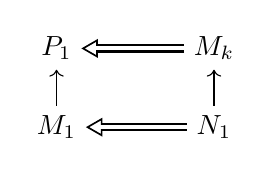
\begin{tikzpicture} %[scale=0.8]
    \node (p1) at (0,1) {\(P_1\)};
    \node (m3) at (2,1) {\(M_k\)};
    \node (m1) at (0,0) {\(M_1\)};
    \node (n1) at (2,0) {\(N_1\)};
    \draw [->] (m1) -- (p1);
    \draw [->] (n1) -- (m3);
    \draw [vecArrow] (m3) -- (p1);
    \draw [vecArrow] (n1) -- (m1);
  \end{tikzpicture}
  \]
  \begin{mdframed}[backgroundcolor=blue!20]
    We have to show in the construction above that matching $h$ defined in~\autoref{eq:matching} allows the dpo rewriting step of $M_k$, that is that the gluing conditions hold.
  \end{mdframed}

  So far, we have a trace $M_2\Rightarrow N_2\cdots M_k\Rightarrow N_2\cdots M_n\Rightarrow N_n$ corresponding to the chain $e_2\prec e'\cdots e_k\prec e''\prec\cdots e_n$ and a transition $P_1\Rightarrow M_k$. The last step consists in "swaping" the transition $P_1\Rightarrow M_k$ at the beginning of the trace, to obtain a trace $M_1\Rightarrow M_2\Rightarrow N_2\cdots M_n\Rightarrow N_n$.

  %% We proceed by induction on the trace $M_2\Rightarrow N_2\cdots M_k\Rightarrow N_2\cdots M_n\Rightarrow N_n$.
  %% Let us consider one step of swapping: let $M_j\overset{e_j}{\Rightarrow} M_{j+1}$ and $P_j\overset{e_1}{\Rightarrow}M_{j+1}$ where $2\leq j\leq k-1$.
  %% \[
  %% \begin{tikzpicture} %[scale=0.8]
  %%   \node (m2) at (0,1) {\(M_2\)};
  %%   \node (dots) at (2,1) {\(\cdots\)};
  %%   \node (mj) at (4,1) {\(M_j\)};
  %%   \node (mj1) at (6,1) {\(M_{j+1}\)};
  %%   \node (dots2) at (8,1) {\(\cdots\)};
  %%   \node (mk) at (10,1) {\(M_k\)};
  %%   \node (pk) at (0,0) {\(P_k\)};
  %%   \node (pkj1) at (2,0) {\(P_{k-j-1}\)};
  %%   \node (pkj) at (4,0) {\(P_{k-j}\)};
  %%   \node (p1) at (8,0) {\(P_{1}\)};
  %%   \draw [vecArrow] (m2) -- (dots);
  %%   \draw [vecArrow] (dots) -- (mj);
  %%   \draw [vecArrow] (mj) -- (mj1);
  %%   \draw [vecArrow] (mj1) -- (dots2);
  %%   \draw [vecArrow] (dots2) -- (mk);
  %%   \draw [vecArrow] (pk) -- (dots);
  %%   \draw [vecArrow] (pkj1) -- (mj);
  %%   \draw [vecArrow] (pkj) -- (mj1);
  %%   \draw [vecArrow] (p1) -- (mk);
  %% \end{tikzpicture}
  %% \]

  The construction of~\autoref{lemm:linear_to_trace} is minimal w.r.t. the choice of decoration and linear extension, in the sense that each graph in the construction is the result of a pushout.

\end{proof}




\newpage

\begin{lemma}[Refinement of a poset for trace reconstruction]
  \label{lem:rewrite_concurrent}
  Let $s=(E,\tleq,\labl)$ be a poset and
  %let $(E,\sqsubset,\labl)\in \decor(s)$ be a decoration of $s$ and
  let $(E,\sqsubset,\labl,\fp)$ be a refinement of $s$.

  Let $e_1,e_2\in E$ be two incomparable events such that
  $\fp(e_1) = M_1\overset{m_1,p_1}{\Rightarrow} M_1'$ and $\fp(e_2) = M_2\overset{m_2,p_2}{\Rightarrow} M_2'$.

  We have the following additional contraint on the refinement of $s$:
  \begin{enumerate}
  \item if the two productions are co-initial, i.e. $M_1\iso M_2$ then there exists $M'$ such that the diagram commutes
  \[
  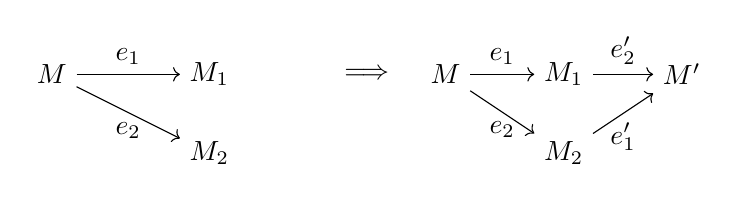
\begin{tikzpicture} %[scale=0.8]
    \node (m2) at (0,0) {\(M_2\)};
    \node (m1) at (0,1) {\(M_1\)};
    \node (m) at (-2,1) {\(M\)};
    \node (implies) at (2,1) {\(\implies\)};
    \node (mm2) at (4.5,0) {\(M_2\)};
    \node (mm1) at (4.5,1) {\(M_1\)};
    \node (n) at (6,1) {\(M'\)};
    \node (mm) at (3,1) {\(M\)};
    \draw [->] (m) -- node [left,above] {\(e_1\)} (m1);
    \draw [->] (m) -- node [left,below] {\(e_2\)} (m2);
    \draw [->] (mm) -- node [left,above] {\(e_1\)} (mm1);
    \draw [->] (mm) -- node [left,below] {\(e_2\)} (mm2);
    \draw [->] (mm1) -- node [left,above] {\(e_2'\)} (n);
    \draw [->] (mm2) -- node [left,below] {\(e_1'\)} (n);
  \end{tikzpicture}
  \]
  Moreover, for any graph $M''$ such that $M''\emb M_1$ then $M''\emb M'$.
  \item if the two productions are co-final, i.e. $M_1'\iso M_2'$ then there exists $M'$ such that the diagram commutes
  \[
  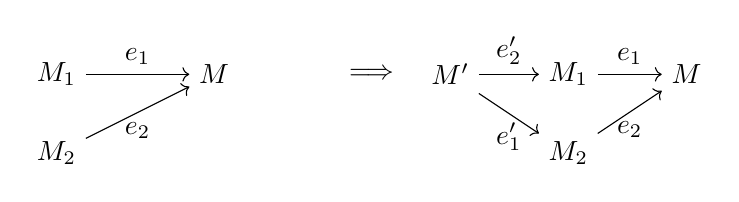
\begin{tikzpicture} %[scale=0.8]
    \node (m2) at (-2,0) {\(M_2\)};
    \node (m1) at (-2,1) {\(M_1\)};
    \node (m) at (0,1) {\(M\)};
    \node (implies) at (2,1) {\(\implies\)};
    \node (mm2) at (4.5,0) {\(M_2\)};
    \node (mm1) at (4.5,1) {\(M_1\)};
    \node (n) at (3,1) {\(M'\)};
    \node (mm) at (6,1) {\(M\)};
    \draw [->] (m1) -- node [left,above] {\(e_1\)} (m);
    \draw [->] (m2) -- node [left,below] {\(e_2\)} (m);
    \draw [->] (mm1) -- node [left,above] {\(e_1\)} (mm);
    \draw [->] (mm2) -- node [left,below] {\(e_2\)} (mm);
    \draw [->] (n) -- node [left,above] {\(e_2'\)} (mm1);
    \draw [->] (n) -- node [left,below] {\(e_1'\)} (mm2);
  \end{tikzpicture}
  \]
  Moreover, for any graph $M''$ such that $M''\emb M_1$ then $M''\emb M'$.
  \end{enumerate}
\end{lemma}
\begin{proof}
  \begin{enumerate}
  \item Let $\labl(e_1)=L_1\action R_1$ and $\labl(e_2)=L_2\action R_2$ be the labels of the two events.
    Then there exists an event $e_3$ such that $e_3\subseteq_{O_1} e_1$ and $e_3\subseteq_{O_2} e_2$. We can assume without loss of generality, that $e_3$ is the only such event (in the cover relation with $e_1$ and $e_2$). Let us show that we can rewrite $M_1'$ using rule $\labl(e_2)$ and obtain $M'$ such that $M_1\overset{e_1}{\Rightarrow} M_1'$ and $M_1'\overset{e_2'}{\Rightarrow} M_2'$ are sequentially independent.
     Let us consider only the poset restricted to events $\{e_1,e_2,e_3\}$. We have that, in the following diagram, there exists a morphism $L_2\to D'$ that commutes.
     \[
     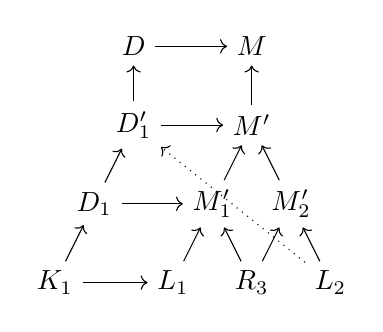
\begin{tikzpicture} %[scale=0.8]
       \node (k1) at (0,0) {\(K_1\)};
       \node (l1) at (1.5,0) {\(L_1\)};
       \node (r3) at (2.5,0) {\(R_3\)};
       \node (l2) at (3.5,0) {\(L_2\)};
       \node (m1) at (2,1) {\(M_1'\)};
       \node (m2) at (3,1) {\(M_2'\)};
       \node (d1) at (0.5,1) {\(D_1\)};
       \node (d1p) at (1,2) {\(D_1'\)};
       \node (m1p) at (2.5,2) {\(M'\)};
       \node (d) at (1,3) {\(D\)};
       \node (m) at (2.5,3) {\(M\)};
       \draw [->] (k1) -- (l1);
       \draw [->] (k1) -- (d1);
       \draw [->] (d1) -- (d1p);
       \draw [->] (d1) -- (m1);
       \draw [->] (d1p) -- (d);
       \draw [->] (d1p) -- (m1p);
       \draw [->] (d) -- (m);
       \draw [->] (l1) -- (m1);
       \draw [->] (r3) -- (m1);
       \draw [->] (r3) -- (m2);
       \draw [->] (l2) -- (m2);
       \draw [->] (m2) -- (m1p);
       \draw [->] (m1) -- (m1p);
       \draw [->] (m1p) -- (m);
       \draw [dotted,->] (l2) -- (d1p);
     \end{tikzpicture}
     \]

     Using the corollar of~\autoref{lem:subposet} if there is no such morphism then events are sequential dependent in the original trace. From~\autoref{def:abstraction}, one has that $e_1 < e_2$, which contradicts the hypothesis.

     If there exists a morphism $L_2\to D'$ that commutes then, using~\autoref{lem:subposet} there is a morphism from $L_2\to D$ that commutes.
     Lastly we use~\autoref{church_rosser} which from such a morphism, infers that $M\overset{e_1}{\Rightarrow} M_1'$ and $M\overset{e_2}{\Rightarrow} M_2'$ are parallel independent.

  \item As we are using DPO rewriting, this case is similar to the first.
  \end{enumerate}
\end{proof}


\begin{definition}[Concretisation of a poset]
  \label{def:concretisation}
  Given a set of posets $\mathcal{S}$ let us define the concretisation function $\gamma:\mathcal{S}\subseteq\Theta$ that sends a poset to a set of traces.
  \begin{itemize}
  \item For $s\in\mathcal{S}$, let $\overline{s}\in\decor(s)$ be a decorated poset.
    We define the refinement of a decorated poset $\mathit{refine}(\overline{s}) = \{E,\sqsubset,\labl,\bp\}$, where $\overline{s} = \{E,\sqsubset,\labl\}$.
  \item For every pair of concurrent events in $\mathit{refine}(\overline{s})$ close out the diagram using~\autoref{lem:rewrite_concurrent}. Denote $S$ a diagram that is closed with respect to the concurrent events. Then define $\gamma$, the concretisation function, as a set of traces, where each trace is a path in the diagram $S$:
    \[
    \gamma(s) = \{ t : t\text{ is a path in }S\text{ and }S\text{ is one the closed diagrams of }\mathit{refine}(\decor(s))\}.
    \]
  \end{itemize}
\end{definition}

\begin{example}
  We complete the refined poset of the left by applying~\autoref{lem:rewrite_concurrent} to obtain the diagram on the right:
  \[
  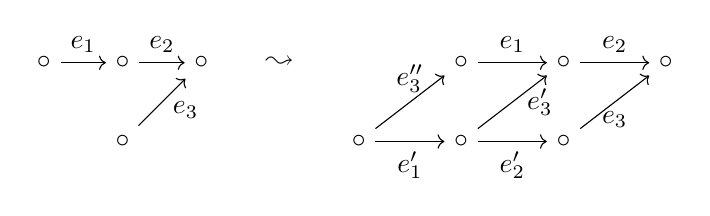
\begin{tikzpicture} %[scale=0.8]
  \node (n2) at (-1,1) {\(\circ\)};
  \node (m2) at (0,0) {\(\circ\)};
  \node (m1) at (0,1) {\(\circ\)};
  \node (n) at (1,1) {\(\circ\)};
  \node (implies) at (2,1) {\(\leadsto\)};
  \node (mm2) at (5.6,0) {\(\circ\)};
  \node (mm1) at (5.6,1) {\(\circ\)};
  \node (nn) at (6.9,1) {\(\circ\)};
  \node (mm) at (4.3,0) {\(\circ\)};
  \node (nn1) at (3,0) {\(\circ\)};
  \node (nn2) at (4.3,1) {\(\circ\)};
  \node (text) at (0.8,0.4) {\(e_3\)};
  \node (text1) at (5.3,0.5) {\(e_3'\)};
  \draw [->] (n2) -- node [left,above] {\(e_1\)} (m1);
  \draw [->] (m1) -- node [left,above] {\(e_2\)} (n);
  \draw [->] (m2) -- (n);
  \draw [->] (nn2) -- node [left,above] {\(e_1\)} (mm1);
  \draw [->] (mm1) -- node [left,above] {\(e_2\)} (nn);
  \draw [->] (mm2) -- node [left,below] {\(e_3\)} (nn);
  \draw [->] (mm) -- node [left,below] {\(e_2'\)} (mm2);
  \draw [->] (mm) -- (mm1);
  \draw [->] (nn1) -- node [above] {\(e_3''\)} (nn2);
  \draw [->] (nn1) -- node [left,below] {\(e_1'\)} (mm);
\end{tikzpicture}
\]
\end{example}


\begin{theorem}
\label{th:correction}
  $\theta\subseteq \gamma(\alpha(\theta))$.
\end{theorem}
\begin{proof}
    \begin{mdframed}[backgroundcolor=blue!20]
    to do
  \end{mdframed}
\end{proof}

\begin{remark}[Adding inhibition]
  We can change definition~\autoref{def:abstraction} in order to construct posets with the additional relation of inhibition between events:
  \[
  e_i \dashv e_j \iff t_i \dashv t_j \text{ and } \alpha(t_i)=e_i, \alpha(t_j)=e_j
  \]
  Inhibition doesn't change the decoration and refinement of a poset but can make the concretisation function "more precise". In~\autoref{def:concretisation} we have to additionally remove any path in $\gamma(\alpha(\theta))$ that has two events $e_1$ followed by $e_2$ such that $e_1\dashv e_2$.
\end{remark}


%Let us first give an example of a refinement of a poset and then introduce all notions we need formally.
\begin{example}
\label{ex:e1e2e3}
Let us consider the poset $(\{e_1,e_2,e_3,e_4\},\sqsubset)$ where $e_1\sqsubset_{O_1}e_2\sqsubset_{O_2}e_3$, $e_4\sqsubset_{O_4}e_3$ and $\labl(e_1)=r_1$, $\labl(e_2)=r_2$, $\labl(e_3)=r_3$, $\labl(e_4)=r_4$.

First we refine $r_2$ using the relation $r_1\redl{+}_{O_1} r_2$, (as we have seen in~\autoref{def:low_res}):
\[
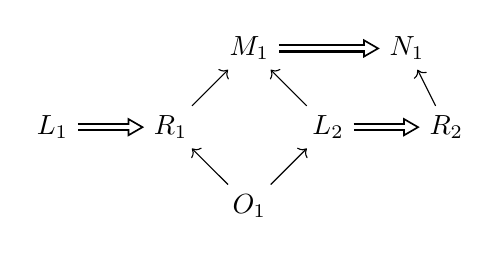
\begin{tikzpicture} %[scale=0.8]
  \node (o1) at (0,-1) {\(O_1\)};
  \node (m1) at (0,1) {\(M_1\)};
  \node (n1) at (2,1) {\(N_1\)};
  \node (r1) at (-1,0) {\(R_1\)};
  \node (l1) at (-2.5,0) {\(L_1\)};
  \node (l2) at (1,0) {\(L_2\)};
  \node (r2) at (2.5,0) {\(R_2\)};
  \draw [->] (o1) -- (r1);
  \draw [->] (o1) -- (l2);
  \draw [->] (r1) -- (m1);
  \draw [->] (r2) -- (n1);
  \draw [->] (l2) -- (m1);
  \draw [vecArrow] (l1) -- (r1);
  \draw [vecArrow] (m1) -- (n1);
  \draw [vecArrow] (l2) -- (r2);
\end{tikzpicture}
\]
We apply a rewriting step to $M_1$ using rule $r_2$ to obtain $N_2$. We refine then $r_3$ using $N_2$ (this step is formally defined in~\autoref{def:seq_comb}):
\[
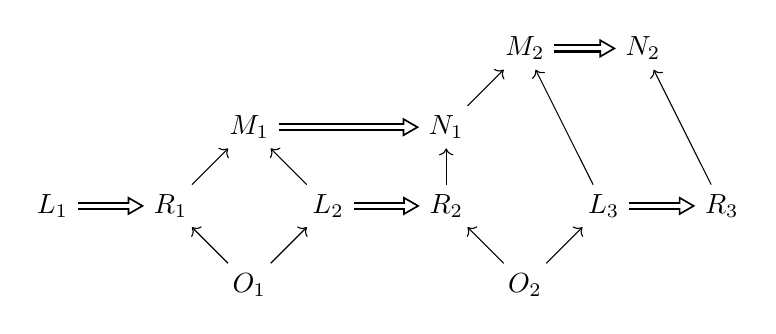
\begin{tikzpicture} %[scale=0.8]
  \node (o1) at (0,-1) {\(O_1\)};
  \node (m1) at (0,1) {\(M_1\)};
  \node (r1) at (-1,0) {\(R_1\)};
  \node (l1) at (-2.5,0) {\(L_1\)};
  \node (l2) at (1,0) {\(L_2\)};
  \node (r2) at (2.5,0) {\(R_2\)};
  \node (o2) at (3.5,-1) {\(O_2\)};
  \node (l3) at (4.5,0) {\(L_3\)};
  \node (r3) at (6,0) {\(R_3\)};
  \node (m2p) at (2.5,1) {\(N_1\)};
  \node (n) at (3.5,2) {\(M_2\)};
  \node (n2) at (5,2) {\(N_2\)};
  \draw [->] (o1) -- (r1);
  \draw [->] (o1) -- (l2);
  \draw [->] (r1) -- (m1);
  \draw [->] (l2) -- (m1);
  \draw [->] (o2) -- (r2);
  \draw [->] (o2) -- (l3);
  \draw [->] (l3) -- (n);
  \draw [->] (m2p) -- (n);
  \draw [->] (r2) -- (m2p);
  \draw [->] (r3) -- (n2);
  \draw [vecArrow] (l1) -- (r1);
  \draw [vecArrow] (l2) -- (r2);
  \draw [vecArrow] (l3) -- (r3);
  \draw [vecArrow] (m1) -- (m2p);
  \draw [vecArrow] (n) -- (n2);
\end{tikzpicture}
\]
Let us now integrate $e_4\sqsubset_{O_4} e_3$ in the sequence. Let $R_4\lemb M_3\remb L_3$ be the cospan obtained from $\labl(e_4)\redl{+}_O\labl(e_3)$.
We combine $M_2$ and $M_3$ using $L_3$ (concurrent combinator is formally introduced in~\autoref{def:conc_comb}):
\[
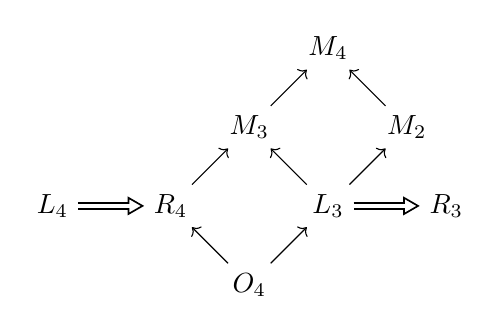
\begin{tikzpicture} %[scale=0.8]
  \node (l4) at (0.5,0) {\(L_4\)};
  \node (r4) at (2,0) {\(R_4\)};
  \node (o4) at (3,-1) {\(O_4\)};
  \node (m4) at (3,1) {\(M_3\)};
  \node (l3) at (4,0) {\(L_3\)};
  \node (r3) at (5.5,0) {\(R_3\)};
  \node (m2p) at (5,1) {\(M_2\)};
  \node (n) at (4,2) {\(M_4\)};
  \draw [->] (o4) -- (r4);
  \draw [->] (o4) -- (l3);
  \draw [->] (r4) -- (m4);
  \draw [->] (l3) -- (m4);
  \draw [->] (m4) -- (n);
  \draw [->] (m2p) -- (n);
  \draw [->] (l3) -- (m2p);
  \draw [vecArrow] (l4) -- (r4);
  \draw [vecArrow] (l3) -- (r3);
\end{tikzpicture}
\]
The refinement of our poset is then the following set of transitions:
\[
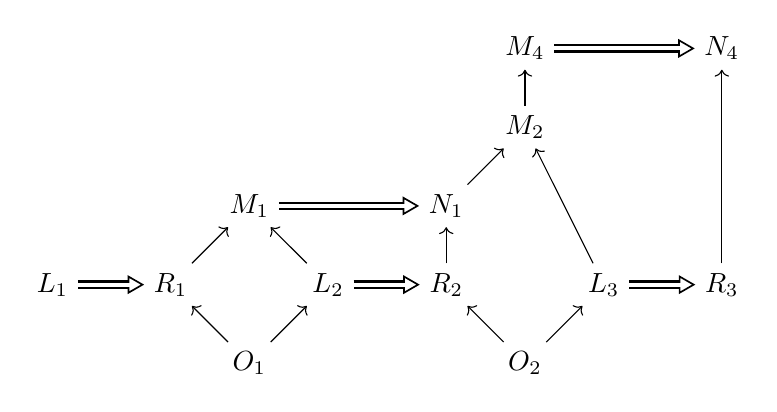
\begin{tikzpicture} %[scale=0.8]
  \node (o1) at (0,-1) {\(O_1\)};
  \node (m1) at (0,1) {\(M_1\)};
  \node (r1) at (-1,0) {\(R_1\)};
  \node (l1) at (-2.5,0) {\(L_1\)};
  \node (l2) at (1,0) {\(L_2\)};
  \node (r2) at (2.5,0) {\(R_2\)};
  \node (o2) at (3.5,-1) {\(O_2\)};
  \node (l3) at (4.5,0) {\(L_3\)};
  \node (r3) at (6,0) {\(R_3\)};
  \node (n1) at (2.5,1) {\(N_1\)};
  \node (m2) at (3.5,2) {\(M_2\)};
  \node (m4) at (3.5,3) {\(M_4\)};
  \node (n4) at (6,3) {\(N_4\)};
  \draw [->] (o1) -- (r1);
  \draw [->] (o1) -- (l2);
  \draw [->] (r1) -- (m1);
  \draw [->] (l2) -- (m1);
  \draw [->] (o2) -- (r2);
  \draw [->] (o2) -- (l3);
  \draw [->] (l3) -- (m2);
  \draw [->] (n1) -- (m2);
  \draw [->] (r2) -- (n1);
  \draw [->] (r3) -- (n4);
  \draw [vecArrow] (l1) -- (r1);
  \draw [vecArrow] (l2) -- (r2);
  \draw [vecArrow] (l3) -- (r3);
  \draw [vecArrow] (m1) -- (n1);
  \draw [->] (m2) -- (m4);
  \draw [vecArrow] (m4) -- (n4);
\end{tikzpicture}
\]

%% Lastly we have to propagate $M_4$ backwards to events $e_1$, $e_2$ and $e_4$.
%% \[
%% \begin{tikzpicture} %[scale=0.8]
%%   \node (o1) at (0,-1) {\(O_1\)};
%%   \node (m1) at (0,1) {\(M_1\)};
%%   \node (r1) at (-1,0) {\(R_1\)};
%%   \node (l1) at (-2.5,0) {\(L_1\)};
%%   \node (l2) at (1,0) {\(L_2\)};
%%   \node (r2) at (2.5,0) {\(R_2\)};
%%   \node (o2) at (3.5,-1) {\(O_2\)};
%%   \node (l3) at (4.5,0) {\(L_3\)};
%%   \node (r3) at (6,0) {\(R_3\)};
%%   \node (n1) at (2.5,1) {\(N_1\)};
%%   \node (m2) at (3.5,2) {\(M_2\)};
%%   \node (n2) at (6,2) {\(N_2\)};
%%   \node (m6) at (-2.5,3) {\(M_6\)};
%%   \node (m5) at (0,3) {\(M_5\)};
%%   \node (m4) at (3.5,3) {\(M_4\)};
%%   \node (n4) at (6,3) {\(N_4\)};
%%   \draw [->] (o1) -- (r1);
%%   \draw [->] (o1) -- (l2);
%%   \draw [->] (r1) -- (m1);
%%   \draw [->] (l2) -- (m1);
%%   \draw [->] (o2) -- (r2);
%%   \draw [->] (o2) -- (l3);
%%   \draw [->] (l3) -- (m2);
%%   \draw [->] (n1) -- (m2);
%%   \draw [->] (r2) -- (n1);
%%   \draw [->] (r3) -- (n2);
%%   \draw [vecArrow] (l1) -- (r1);
%%   \draw [vecArrow] (l2) -- (r2);
%%   \draw [vecArrow] (l3) -- (r3);
%%   \draw [vecArrow] (m1) -- (n1);
%%   \draw [vecArrow] (m2) -- (n2);
%%   \draw [->] (n2) -- (n4);
%%   \draw [->] (m2) -- (m4);
%%   \draw [->] (m1) -- (m5);
%%   \draw [->] (l1) -- (m6);
%%   \draw [vecArrow] (m4) -- (n4);
%%   \draw [vecArrow] (m4) -- (m5);
%%   \draw [vecArrow] (m5) -- (m6);
%% \end{tikzpicture}
%% \]
%% The refinement of our poset is then the set of transitions
%% \[
%% \begin{tikzpicture} %[scale=0.8]
%%   \node (m6) at (0,1) {\(M_6\)};
%%   \node (m5) at (1.5,1) {\(M_5\)};
%%   \node (m4) at (3,1) {\(M_4\)};
%%   \node (n4) at (4.5,1) {\(N_4\)};
%%   \node (m7) at (1.5,0) {\(M_7\)};
%%   \draw [vecArrow] (m4) -- (n4);
%%   \draw [vecArrow] (m5) -- (m4);
%%   \draw [vecArrow] (m6) -- (m5);
%%   \draw [vecArrow] (m7) -- (m4);
%% \end{tikzpicture}
%% \]
%% where $M_7$ is obtained by a rewriting of $M_4$ using rule $r_4$.
\end{example}

\begin{definition}[Refinement of a rule~\cite{information_carriers}]
  Let $r:L{\Rightarrow} R$ be a rule and let $m:L\emb M$ be a matching in a graph $M$. The production $M\overset{m,r}{\Rightarrow} N$ obtained by DPO rewriting of $M$ using the rule $r$ is called a \emph{refinement} of $r$.
\end{definition}

\begin{definition}[Refinement of a poset]
  \label{def:ref_poset}
  Given a poset $s=(E,<,\labl)$ of graph rewriting events, the \emph{refinement} of $s$, is a bijection $\imath$ between events $e\in E$ and transitions $M\overset{m,p}{\Rightarrow} M'$ such that
  \begin{itemize}
  \item the label of an event is rule in the transition: $\labl(e)=p$;
  \item for all $e_1,e_2\in E$, if $e_1<e_2$ and $\imath(e_1) = M_1\overset{m_1,p_1}{\Rightarrow} M_1'$, $\imath(e_2) =M_2\overset{m_2,p_2}{\Rightarrow} M_2'$ then $M_1'\emb M_2$.
  \end{itemize}
\end{definition}

%Before giving the construction of a refinement $(M_i\overset{m_i,p_i}{\Rightarrow} M_{i+1})_{e_i\in E}$ let us first introduce some combinators of contexts.

%% \begin{definition}[Propagate a context]
%%   \label{def:propagate}
%%   Given a sequence $M_1{\Rightarrow} M_2\cdots {\Rightarrow} M_n\cdots {\Rightarrow} M_{m}$ and a graph $M_{n}'$ with $M_n\emb M_{n}'$ define the \emph{propagation} of $M_{n}'$ as the sequence  $M_1'{\Rightarrow} M_2'\cdots {\Rightarrow} M_n'\cdots {\Rightarrow} M_{m}'$ where
%%   \begin{itemize}
%%   \item $M_i'$, for $i<n$, is obtained by the reverse of the production $M_i\Rightarrow M_{i+1}$ applied to the new contexts;
%%   \item $M_i'$, for $n<i\leq m$, is obtained by the production $M_i\Rightarrow M_{i+1}$ applied to the new contexts.
%%   \end{itemize}
%% \end{definition}

\begin{definition}[Sequential combinator]
\label{def:seq_comb}
  Let $M\Rightarrow N$ and $L\Rightarrow R$ be two productions such that there exists $N\remb O \lemb L$ a cospan.
  Define the sequential combinator as follows:
  \[
  (M\overset{m,p}{\Rightarrow}N)\oplus_O (L\Rightarrow R) = M'\overset{m',p'}{\Rightarrow}N'
  \]
  where $N\emb M' \remb L$ is the pushout of the cospan $N\remb O \lemb L$ and $N'$ is obtained by a DPO rewriting of $M'$ by the production $L\Rightarrow R$:
  \[
  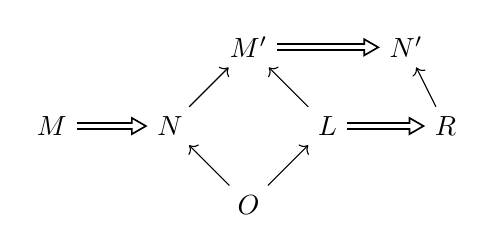
\begin{tikzpicture} %[scale=0.8]
    \node (o) at (0,-1) {\(O\)};
    \node (mp) at (0,1) {\(M'\)};
    \node (m) at (-2.5,0) {\(M\)};
    \node (n) at (-1,0) {\(N\)};
    \node (l) at (1,0) {\(L\)};
    \node (r) at (2.5,0) {\(R\)};
    \node (np) at (2,1) {\(N'\)};
    \draw [->] (o) -- (n);
    \draw [->] (o) -- (l);
    \draw [->] (n) -- (mp);
    \draw [->] (l) -- (mp);
    \draw [->] (r) -- (np);
    \draw [vecArrow] (m) -- (n);
    \draw [vecArrow] (l) -- (r);
    \draw [vecArrow] (mp) -- (np);
  \end{tikzpicture}
  \]
  We denote $m'$ the morphism $L\to M'$ and $p'$ the production $L\Rightarrow R$.
\end{definition}

\begin{definition}[Wide pushout~\cite{wide}]
The wide pushout of a family of morphisms $(P\to M_i)_i$ consists of a graph $M$ and a family of morphisms $(M_i\to M)_i$ such that the diagram commutes
\[
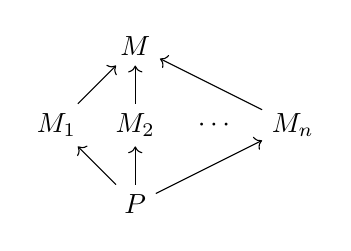
\begin{tikzpicture} %[scale=0.8]
  \node (o) at (0,-1) {\(P\)};
  \node (m1) at (-1,0) {\(M_1\)};
  \node (m2) at (0,0) {\(M_2\)};
  \node (text) at (1,0) {\(\cdots\)};
  \node (mn) at (2,0) {\(M_n\)};
  \node (m) at (0,1) {\(M\)};
  \draw [->] (o) --  (m1);
  \draw [->] (o) --  (m2);
  \draw [->] (o) --  (mn);
  \draw [->] (m1) --  (m);
  \draw [->] (m2) --  (m);
  \draw [->] (mn) --  (m);
\end{tikzpicture}
\]
for any other $M'$ and family of morphisms $(M_i\to M')_i$ there exists a unique morphism $M\to M'$ that commutes.

The wide pushout is equivalent to computing the pushout pairwise on $(P\to M_i)_i$.
\end{definition}

\begin{lemma}[Concurrent combinator]
  \label{def:conc_comb}
  Let $(M_i)_{0< i< n}$ be a family of graphs, let $(M'\emb M_i)_{0< i< n}$ be a family of injective morphisms and let $p:L\Rightarrow R$ be a production.
  Define the concurrent combinator as follows:
  \[
  \otimes_{L{\Rightarrow}R}(M_1, M_2,\cdots M_n) = M \overset{m,p}{\Rightarrow} N
  \]
  where $M$ is the wide pushout of the family of morphisms $(L\emb M_i)_i$.

  The morphisms $m_i$, obtained by the composition of $L\emb M_i$ and $M_i\emb M$ are equivalent. We denote $m$ one such morphism.

  The graph $N$ is obtained by a DPO rewriting of $M$ by the production $p$.
\end{lemma}
\begin{proof}
  First we prove that the morphisms $m_i$ obtained by the composition of $M'\emb M_i$  and $M_i\emb M$ are equivalent.
% which follows from the definition of the pushout.
  Secondly we show that the gluing conditions hold for the DPO rewriting of $p$ on $M$ iff they hold for the dpo rewriting of $p$ on all $M_i$. Both follow from $(M_i\to M)_i$ being the wide pushout of $(L\to M_i)_i$.
\end{proof}

\begin{definition}[Refinement propagation]
  \label{def:ref_propagator}
  Let $s=(E,\tleq,\labl)$ be a poset and let $(E,\sqsubset,\labl)\in \decor(s)$ be a decoration of $s$.
  We define a function, called the \emph{forward propagator}, by induction on $s$:
  \begin{align*}
    &\fp(e) = L\Rightarrow R&\text{ if }e\in\text{min}(s)\text{ and }\labl(e) = L\action R\\
    &\fp(e) = M\overset{m,p}{\Rightarrow} N&\text{ where }\forall e_i, e_i\sqsubset_{O_i}e,
    \fp(e_i)\oplus_{O_i}L\Rightarrow R= M_i\overset{m_i,p}{\Rightarrow} N_i\\
    &&\otimes_{\labl(e)}(M_1, M_2, \cdots M_n) = M \overset{m,p}{\Rightarrow} N
    \text{and }\labl(e) = p:L\action R\\
  \end{align*}
\end{definition}

\begin{lemma}
  $(E,\sqsubset,\labl,\fp)$ is a refinement of $(E,<,\labl)$.
\end{lemma}
\begin{proof}
  For the base case we have only to show that, for $\fp(e) = M\overset{m,p}{\Rightarrow} N$, $\labl(e)=p$. This follows from~\autoref{def:seq_comb} and~\autoref{def:conc_comb}.

  For the inductive case, let us consider an event $e$. As above, we have that if $\fp(e) = M\overset{m,p}{\Rightarrow} N$ then $\labl(e)=p$. If there exists $e'$, $e'\sqsubset_O e$ with $\fp(e')= M'\overset{m',p'}{\Rightarrow} N'$ then, from~\autoref{def:ref_propagator} and from~\autoref{def:seq_comb}, there exists $M''$ such that $M'\emb M''$. Moreover, from~\autoref{def:conc_comb}, $M''\emb M$.
\end{proof}

%% \begin{definition}[Refinement propagation]
%%   \label{def:ref_propagator}
%%   Let us define two functions the forward propagator $\fp$, and the backward propagator $\bp$, that map events in a poset $\{E,\sqsubset,\labl\}$ to transitions.
%% We proceed by induction on the transitive and reflexive closure of the cover relation $\sqsubset$ and start with the minimal events for the definition of $\fp$. For the definition of $\bp$ we proceed by induction on the transitive and reflexive closure of the reverse relation $\sqsubset^{-1}$ starting with the maximal events for $\bp$:
%% \begin{align*}
%%   \text{forward propagator}\\
%%   &\fp(e) = \labl(e)&\text{ if }e\in\text{min}(s)\\
%%   &\fp(e) = M\Rightarrow N&\text{ where }\forall e_i, e_i\sqsubset_{O_i}e, \fp(e_i)\oplus_{O_i}\labl(e) = M_i\Rightarrow N_i\\
%%   &&\otimes_{\labl(e)}(M_1, M_2, \cdots M_n) = M \Rightarrow N\\
%%   \\
%%   \text{backward propagator}\\
%%   &\bp(e) = \fp(e)&\text{ if }e\in\text{max}(s)\\
%%   &\bp(e) = M\Rightarrow N&\text{ where }\forall e_i, e\sqsubset_{O_i}e_i, \bp(e_i) = M_i\Rightarrow N_i\\
%%   &&\otimes_{\fp(e)^{-1}}(M_1, M_2, \cdots M_n) = M \Rightarrow N
%% \end{align*}
%% \end{definition}

%% \begin{definition}[Embeddings between transitions]
%%   A transition $M'\overset{m',p}\Rightarrow N'$ embeds into a transition $M\overset{m,p}\Rightarrow N$ if there exists a morphism $h:M'\to M$ such that the diagram commutes:
%%   \[
%%   \begin{tikzpicture} %[scale=0.8]
%%     \node (d) at (0,2.5) {\(D\)};
%%     \node (m) at (-2,2.5) {\(M\)};
%%     \node (n) at (2,2.5) {\(N\)};
%%     \node (m1) at (-2,1) {\(M'\)};
%%     \node (d1) at (0,1) {\(D'\)};
%%     \node (n1) at (2,1) {\(N'\)};
%%     \node (l) at (-2,-0.5) {\(L\)};
%%     \node (k) at (0,-0.5) {\(K\)};
%%     \node (r) at (2,-0.5) {\(R\)};
%%     \draw [left hook->] (l) -- node [right,midway] {$m'$} (m1);
%%     \draw [left hook->] (r) -- (n1);
%%     \draw [left hook->] (k) -- (d1);
%%     \draw [left hook->] (k) -- (l);
%%     \draw [left hook->] (k) -- (r);
%%     \draw [dotted, left hook->] (m1) -- (m);
%%     \draw [dotted, left hook->] (d1) -- (d);
%%     \draw [dotted, left hook->] (n1) -- (n);
%%     \draw [left hook->] (d1) -- (m1);
%%     \draw [left hook->] (d1) -- (n1);
%%     \draw [left hook->] (d) -- (m);
%%     \draw [left hook->] (d) -- (n);
%%     \draw [left hook->] (l) to [bend left] node [left,midway] {$m$} (m);
%%     \draw [left hook->] (k) to [bend right] (d);
%%     \draw [left hook->] (r) to [bend right] (n);
%%   \end{tikzpicture}
%%   \]
%% \end{definition}

%% \begin{lemma}
%%   \label{lem:subposet}
%%   Let $s'\subseteq s$ be a connected poset (i.e. directed either upwards or downwards). Then
%%   \[\forall e\in s', \bp_{s'}(e)\text{ embeds into }\bp_s(e),\]
%%   where $\bp_s(e)$ is the refinement of~\autoref{def:ref_propagator} applied to $s$.
%%   A \textbf{corollary} is that if two transitions are sequential dependent in $\bp_{s'}$ then they are sequential dependent in $\bp_{s}$.
%% \end{lemma}
%% \begin{proof}
%%   \begin{mdframed}[backgroundcolor=blue!20]
%%     to do
%%   \end{mdframed}
%% \end{proof}


%% \begin{example}[Feedback loops]
%% Let us show how we can interpret negative feedback loops. Let $e_1\in s_1\redl{-} e_2\in s_2$ such that $s_2\subset s_1$. Then $e_2\leq_{s_1} e_2$. However this additional constraint does not change the way we interpret negative influence, that is the influence is realised if there exists $M$ such that the following diagram commutes:
%% \[
%% \begin{tikzpicture} %[scale=0.8]
%%   \node (o) at (0,0) {\(O\)};
%%   \node (n) at (0,2) {\(M\)};
%%   \node (l1) at (-1,0) {\(L_1\)};
%%   \node (l2) at (1,0) {\(L_2\)};
%%   \node (n1) at (-1,1) {\(M_1\)};
%%   \node (n2) at (1,1) {\(M_2\)};
%%   \draw [->] (l1) -- (n1);
%%   \draw [->] (l2) -- (n2);
%%   \draw [->] (o) -- (n1);
%%   \draw [->] (o) -- (n2);
%%   \draw [->] (n1) -- (n);
%%   \draw [->] (n2) -- (n);
%% \end{tikzpicture}
%% \]
%% \end{example}


%\subsection{Refinement of decorated posets}

\begin{lemma}[Update of a decoration after a refinement]
  \label{lem:update_dec}
  Let $(E,\redl{+},\redl{-},\labl)$ be a valid decorated poset and let $e_1$ and $e_2$ be two events such that $e_1\redl{+}_{s_1} e_2$ and $e_2\redl{-}_{s_2} e_1$, for two cospans $s_1$ and $s_2$ possibly empty.
  \begin{enumerate}
  \item If there exists $e_3$ and $s:R_i\remb O \lemb L_3$ such that $e_i\redl{+}_s e_3$ with $i\in\{1,2\}$ then there exists $s':M_2\lemb O'\remb L_3$ such that $\big( M_1\remb K\lemb M_2\big)\redl{+}_{s'} r_3$ and such that the diagram commutes:
    \[
    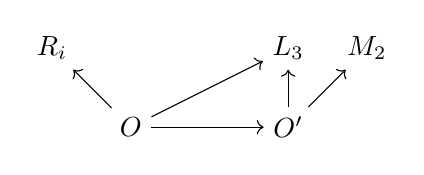
\begin{tikzpicture} %[scale=0.8]
      \node (ri) at (-1,1) {\(R_i\)};
      \node (m2) at (3,1) {\(M_2\)};
      \node (l3) at (2,1) {\(L_3\)};
      \node (o) at (0,0) {\(O\)};
      \node (o1) at (2,0) {\(O'\)};
      \draw [->] (o) -- (o1);
      \draw [->] (o) -- (l3);
      \draw [->] (o1) -- (l3);
      \draw [->] (o) -- (ri);
      \draw [->] (o1) -- (m2);
    \end{tikzpicture}
    \]
    where $\big(\labl(e_1)\otimes_{(s_1\times s_2)} \labl(e_2)\big) = M_1\remb K\lemb M_2$.
  %% \item If there exists $e_3$ and $s:L_i\remb O \lemb L_3$ such that $e_i\redl{-}_s e_3$ with $i\in\{1,2\}$ then there exists $s':M_1\lemb O'\remb L_3$ such that $\big( M_1\remb K\lemb M_2\big)\redl{-}_{s'} r_3$ and such that the diagram commutes:
  %%   \[
  %%   \begin{tikzpicture} %[scale=0.8]
  %%     \node (ri) at (-1,1) {\(L_i\)};
  %%     \node (m2) at (3,1) {\(M_1\)};
  %%     \node (l3) at (2,1) {\(L_3\)};
  %%     \node (o) at (0,0) {\(O\)};
  %%     \node (o1) at (2,0) {\(O'\)};
  %%     \draw [->] (o) -- (o1);
  %%     \draw [->] (o) -- (l3);
  %%     \draw [->] (o1) -- (l3);
  %%     \draw [->] (o) -- (ri);
  %%     \draw [->] (o1) -- (m2);
  %%   \end{tikzpicture}
  %%   \]
  %%   where $\big(\labl(e_1)\otimes_{(s_1\times s_2)} \labl(e_2)\big) = M_1\remb K\lemb M_2$.
  \item If there exists $e_3$ and $s:R_i\remb O \lemb L_3$ such that $e_3\redl{+}_s e_i$ with $i\in\{1,2\}$ then there exists $s':M_2\lemb O'\remb L_3$ such that $r_3\redl{+}_{s'}\big( M_1\remb K\lemb M_2\big)$ and such that the diagram commutes:
    \[
    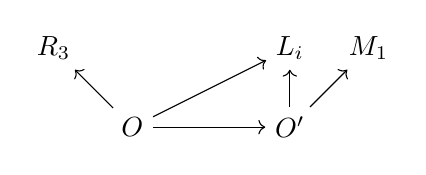
\begin{tikzpicture} %[scale=0.8]
      \node (ri) at (-1,1) {\(R_3\)};
      \node (m2) at (3,1) {\(M_1\)};
      \node (l3) at (2,1) {\(L_i\)};
      \node (o) at (0,0) {\(O\)};
      \node (o1) at (2,0) {\(O'\)};
      \draw [->] (o) -- (o1);
      \draw [->] (o) -- (l3);
      \draw [->] (o1) -- (l3);
      \draw [->] (o) -- (ri);
      \draw [->] (o1) -- (m2);
    \end{tikzpicture}
    \]
    where $\big(\labl(e_1)\otimes_{(s_1\times s_2)} \labl(e_2)\big) = M_1\remb K\lemb M_2$.
  \end{enumerate}
\end{lemma}
\begin{proof}
  \begin{enumerate}
  \item Let us first show the property above for $r_1$.
    We have the following diagram from~\autoref{def:ref_pos_neg_infl}, where $O_3$ is a graph such that $O_1\emb O_3$ and $O_2\emb O_3$.
    \[
    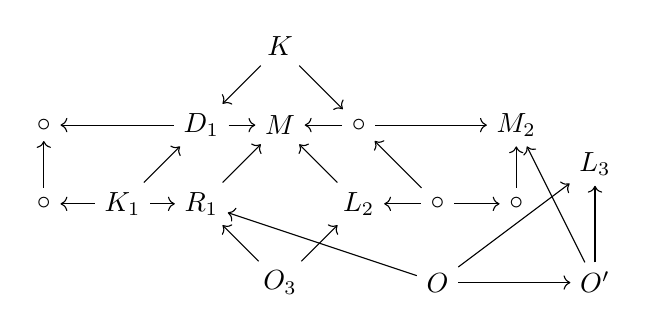
\begin{tikzpicture} %[scale=0.8]
      \node (o) at (0,-1) {\(O_3\)};
      \node (m) at (0,1) {\(M\)};
      \node (d2) at (1,1) {\(\circ\)};
      \node (m2) at (3,1) {\(M_2\)};
      \node (d1) at (-1,1) {\(D_1\)};
      \node (m1) at (-3,1) {\(\circ\)};
      \node (r1) at (-1,0) {\(R_1\)};
      \node (k1) at (-2,0) {\(K_1\)};
      \node (l1) at (-3,0) {\(\circ\)};
      \node (l2) at (1,0) {\(L_2\)};
      \node (k2) at (2,0) {\(\circ\)};
      \node (r2) at (3,0) {\(\circ\)};
      \node (k) at (0,2) {\(K\)};
      \node (l3) at (4,0.5) {\(L_3\)};
      \node (o2) at (2,-1) {\(O\)};
      \node (o1) at (4,-1) {\(O'\)};
      \draw [->] (o) -- (r1);
      \draw [->] (o) -- (l2);
      \draw [->] (r1) -- (m);
      \draw [->] (k1) -- (r1);
      \draw [->] (k1) -- (l1);
      \draw [->] (k1) -- (d1);
      \draw [->] (l1) -- (m1);
      \draw [->] (l2) -- (m);
      \draw [->] (k2) -- (r2);
      \draw [->] (k2) -- (l2);
      \draw [->] (k2) -- (d2);
      \draw [->] (r2) -- (m2);
      \draw [->] (d1) -- (m);
      \draw [->] (d1) -- (m1);
      \draw [->] (d2) -- (m);
      \draw [->] (d2) -- (m2);
      \draw [->] (k) -- (d1);
      \draw [->] (k) -- (d2);
      \draw [->] (o2) -- (o1);
      \draw [->] (o2) -- (l3);
      \draw [->] (o1) -- (l3);
      \draw [->] (o2) -- (r1);
      \draw [->] (o1) -- (m2);
    \end{tikzpicture}
    \]
    We have that $n_1(o(O))\subseteq M$. We distinguish two cases:
    \begin{itemize}
    \item if $n_1(o(O)) \cap m_2(L_2)=\emptyset$ then $f_2^{-1}$ is defined on $n_1(o(O))$. Hence there exists a morphism $o_2:O\emb M_2$ such that $o_2 = g_2 \circ (f_2^{-1}) \circ n_1 \circ o$. Moreover, as $O$ does not embed into $K_1$ (from $e_1\redl{+}_O e_3$), then we can show by contradiction that there is no morphism $O\emb D_1$ nor $O\emb K$ such that the diagram commutes. Therefore we have that there exists $O'$ such that $\labl(e_1)\otimes_{O_1,O_2} \labl(e_2)\redl{+}_{O'} e_3$ and $O\subseteq O'$.
    \item if $n_1(o(O)) \cap m_2(L_2)\neq\emptyset$, then again we distinguish two subcases. A first one is that $f_2^{-1}$ is defined on $n_1(o(O)) \cap m_2(L_2)$, in which case the proof follows as above. Otherwise, we have that there exists $O''\subseteq O$ such that $e_1\redl{+}_{O''} e_2$ and $e_1\redl{+}_{O''} e_3$ which contradicts the contraints on decoration of meets from~\autoref{prop:constraints_poset}.
    \end{itemize}

    The property holds for $r_2$ in a similar manner, except that we use the contraints on decoration of joins from~\autoref{prop:constraints_poset} for the last case.

  \item
    \begin{mdframed}[backgroundcolor=blue!20]
      to do
    \end{mdframed}
  \end{enumerate}
\end{proof}

  Let $e_1$ and $e_2$ be two events of a decorated poset and $s_1,s_2$ be two cospans such that $(\labl(e_1)\otimes_{s_1\otimes s_2} \labl(e_2)) = r_{12}$ is well defined. Moreover, let $e_3$ be an event and $s$ a cospan such that $e_1\redl{+}_s e_3$. We use the notation $\big(e_1\redl{+}_O e_3\big)_{e_1\otimes e_2}$ denotes the set of all decorations $r_{12}\redl{+}_{s'} \labl(e_3)$, where $s'$ is obtained as in~\autoref{lem:update_dec}. We use similar notations for the negative influence and the influences of $e_2$ on $e_3$.

\begin{lemma}[The update is associative]
  \label{lem:assoc}
   Let $e_1,e_2,e_3$ be three events in a decorated poset and $s_1,s_2$ be two cospans such that $e_1\redl{+}_{s_1} e_2\redl{+}_{s_2} e_3$.
   Moreover, let $e_1\oplus_{s_1} e_2 = r_{12}$ and $e_2\oplus_{s_2} e_3 = r_{23}$ be the two refinements.
   Then, for any cospan $s$ such that
   $r_{12}\redl{+}_{s} \labl(e_3)\in\big(e_2\redl{+}_{s_2} e_3\big)_{e_1\otimes e_2}$ there exists a graph $s'$ such that
   $\labl(e_{1})\redl{+}_{s'} r_{23}\in\big(e_1\redl{+}_{s_1} e_2\big)_{e_2\otimes e_3}$ and such that
   \begin{align*}
     (r_1\oplus_{s_1} r_2)\oplus_{s} r_3 \iso r_1\oplus_{s'} (r_2\oplus_{s_3} r_3).
   \end{align*}
\end{lemma}
\begin{mdframed}[backgroundcolor=blue!20]
  \begin{proof}
    to do
  \end{proof}
\end{mdframed}

\begin{mdframed}[backgroundcolor=blue!20]
Adapt \autoref{lem:update_dec} and \autoref{lem:assoc} to inhibition.
\end{mdframed}

\begin{definition}
  Let $e_1,e_2\in E$ be two events of a decorate poset $s$ such that $e_1\redl{+}_{s_1}e_2$, $e_2\redl{-}_{s_2}e_2$ for some $s_1$, $s_2$ possibly empty. Then $\labl(e_1)\otimes_{(s_1\otimes s_2)} r_2=r_{12}$ is well defined.

  Define $s_{(e_1\otimes e_2)} = (E\setminus\{e_1,e_2\}\uplus\{e_{12}\},\overset{+}{\leadsto},\overset{-}{\leadsto},\labl')$ such that
    \begin{align*}
    &\labl'(e)=\labl(e), \forall e,e'\in E\setminus\{e_1,e_2\}\\
    &e\overset{+}{\leadsto}_s e' \iff e\redl{+}_s e', \forall e,e'\in E\setminus\{e_1,e_2\}\\
    &e\overset{-}{\leadsto}_s e' \iff e\redl{-}_s e', \forall e,e'\in E\setminus\{e_1,e_2\}\\
    &\labl'(e_{12}) = r_{12}\\
    &e_{12}\overset{+}{\leadsto}_s e \iff r_{12}\redl{+}_s \labl(e)\in \big(e_i \redl{+}_{s'} e\big)_{e_1\otimes e_2}\\
   % \text{ and }e_i\redl{+}_{O'} e\\
    &e_{12}\overset{-}{\leadsto}_s e \iff r_{12}\redl{-}_s \labl(e)\in \big(e_i \redl{-}_{s'} e\big)_{e_1\otimes e_2}\\
    %\text{ and }e_i\redl{-}_{O'} e\\
  \end{align*}
\end{definition}
%% \begin{lemma}
%%   Let $\underline s = (E,\seq,\redl{+},\redl{-},\labl)$ be a linear extension of a decorated poset $s$. For any two events $e_1,e_2$ such that $\big(s \big)_{e_1\otimes e_2}$ is well defined, $\big(\underline s \big)_{e_1\otimes e_2}$ is a linear extension of $\big(s \big)_{e_1\otimes e_2}$.
%% \end{lemma}

\begin{lemma}
  If $s$ is a valid decorated poset then for any two events $e_1,e_2$ in $s$, $s_{(e_1\otimes e_2)}$ is also a valid decorate poset.
\end{lemma}


\begin{definition}[Refinement of a poset]
  \label{def:ref_poset}
  Let $\underline s=(E,\seq\redl{+},\redl{-},\labl)$ be a linear extension of a decorated poset $s$.
  Define $\mathtt{Ref}(\underline s)$ as follows
  \begin{align*}
    \mathtt{Ref}(\underline s) =&
    \mathtt{Ref}(\underline s')\text{ if }\exists e_1,e_2\in E, e_1\neq e_2, e_1\prec e_2, e_1\redl{+}e_2
    \text{ and }\underline s'=\big(\underline s\big)_{e_1\otimes e_2}
    \\
    &\underline s\text{ otherwise.}\\
  \end{align*}
\end{definition}

%% \section{Logic on posets}
\label{sec:posets}

%\subsection{Category of posets}

%% \begin{definition}[Poset]
%%   A poset $s=\{E,\leq\}$ is a finite set of events $E$ and a partial order on events $\leq\subseteq E\times E$. The \emph{cover} relation on events $\cover\subseteq E\times E$ is the transitive reduction of $\leq$.
%%   We use the predicates $\text{min}(s)$ and $\text{max}(s)$ to retrieve the minimal and maximal events, respectively.
%%   A labeled poset $s=\{E,\leq,\labl\}$ is a set with an additional labelling function $\labl$ defined on events.
%% \end{definition}

\begin{definition}[Augmented poset]
  \label{def:poset}
  An \emph{augmented poset} $s=(E,\prec,\dashv)$ is a set of events $E$ equipped with two binary relations on events: \emph{precedence} denoted $\prec$, and \emph{inhibition} denoted $\dashv$, such that the following hold:
  \begin{itemize}
  \item \emph{events are not pairwise inhibiting:}
    $\forall e_1,e_2\in s$, $e_1\dashv^{\star} e_2\implies \neg(e_2 \dashv^{\star} e_1)$;
  \item \emph{events cannot inhibit their succesors:}
    $\forall e_1,e_2\in s$, $e_1\leq e_2\implies \neg(e_1 \dashv^{\star} e_2)$;
  \end{itemize}
  where $\leq$ is the transitive and reflexive closure of $\prec$ and $\dashv^{\star}$ is the transitive and closure of $\dashv$.

  A labeled poset $s=(E,\prec,\dashv,\labl)$ is an augmented poset with an additional labelling function $\labl:E\to \textit{labels}$ defined on events.
  We use the predicates $\text{min}(s)$ and $\text{max}(s)$ to retrieve the minimal and maximal events, respectively.
  A poset is \emph{directed} when every pair of events has an upper bound.
\end{definition}

\begin{definition}[Morphisms on posets\footnote{Augmented posets and morphisms form a category.}]
  Given two posets $s_1$, $s_2$ a morphism $f:s_1\to s_2$ is a total function on events that preserves labels and preserves the precedence and inhibition relations. We denote $s_1\iso s_2$ whenever there is an isomorphism between $s_1$ and $s_2$.
%  A morphisms on posets is \emph{injective}, denoted $s_1\emb s_2$, when it is injective on events.
\end{definition}

\subsection{Grammar}

Let $\mathcal{R}$ be a set of labels, $\mathcal{S}$ be a set of posets and let $\varepsilon = \cup_{s_i\in S} E_i$ be the set of events in $\mathcal{S}$, where $E_i$ is the set of events in $s_i$.
We denote $A,B$ elements of $\mathcal{R}$ and $s$ elements of $\mathcal{S}$.

\begin{align*}
  x ::= & x^e ~|~ x^s & \tag{variables on events and posets} \\
  t^s ::= & x^s ~|~ s ~|~ \text{min}(t^s) ~|~ \text{max}(t^s) &\tag{terms on posets} \\
  t^e ::= & x^e ~|~ e & \tag{terms on events}\\
  t ::= & t^s ~|~ t^e & \tag{terms}\\
  \\
  \varphi ::= & \exists x.\varphi(x) ~|~ \forall x.\varphi(x) ~|&\tag{quantifiers}\\
  & \neg \varphi ~|~\varphi_1 \wedge \varphi_2~|&\tag{logical connectors}\\
  & t^e\in t^s ~|~ \labl(t^e) = A ~|~ t^e_1 <_{t^s} t^e_2 ~|~ t^e_1 \tleq_{t^s} t^e_2 ~|~ t^e_1\in t^s_1 \dashv t^e_2\in t^s_2~|~ t^s_1 = t^s_2 ~|~ t^s_1\subseteq t^s_2
  & \tag{predicates}\\
\end{align*}

We define the logical connectors $\vee$, $\implies$ in the usual manner.

\subsection{Interpretation}

We interpret the logic on the domain of events and posets.

%an interpretation is the link between syntax and semantics. The functions and predicates are interpreted as their corresponding operations on events and posets.
%The predicates $s_1 = s_2$ and $s_1\subseteq s_2$ are interpreted using isomorphisms and embedings in the category of posets defined below (\autoref{sec:posets}).

%The interpretation of $s_1\cap s_2$ is the set $s_1\otimes s_2$, introduced in \autoref{def:posets_otimes}.
The predicate $\dashv$ can be seen as a predicate that relates events in different posets. Our interpretation in the restrainted case of graph rewriting systems (and in Kappa) will be that of inhibition (\autoref{def:ref_neg_infl}), as we will see in the next sections. The remaining of function and predicates used in our logic have a standard interpretation.

A \emph{valuation} for $\varphi$ is a function
$v:\text{fv}(\varphi)\to\mathcal{E}\uplus\mathcal{S}$
from the set of free variables of $\varphi$ to the set of events and posets.
%
The evaluation of $\varphi$ is defined below, where a valuation function is needed for the set of free variables of $\varphi$.
%We use two functions $\enct$ to evaluate terms and $\enc$ to evaluate formulas.
\begin{align*}
  \enc{\forall x^s.\varphi}_{v} &= T \iff\text{ for all }s\in\mathcal{S}, \enc{\varphi(s/x)}_{v} = T\\
  \enc{\exists x^s.\varphi}_{v} &= T \iff\text{ for some }s\in\mathcal{S}, \enc{\varphi(s/x)}_{v} = T\\
  \enc{\neg\varphi}_v &= \neg\enc{\varphi} \\
  \enc{\varphi_1\wedge\varphi_2}_v &= \enc{\varphi_1}_v\wedge\enc{\varphi_2}_v\\
  \enc{t^e\in t^s}_v &= T\iff\enct{t^e}_v\in\enct{t^s}_v\\
  \enc{\labl(t^e) = A}_v &= T\iff\labl(\enct{t^e}_v)=A\\
  \enc{t^e_1 <_{t^s} t^e_2} &= T\iff e_1 <_s e_2\text{ where }e_1 = \enct{t^e_1}_v,e_2 = \enct{t^e_2}_v,s = \enct{t^s}_v\\
  \enc{t^e_1 \tleq_{t^s} t^e_2} &= T\iff e_1 \tleq_s e_2\text{ where }e_1 = \enct{t^e_1}_v,e_2 = \enct{t^e_2}_v,s = \enct{t^s}_v\\
  \enc{t^e_1\in t^s_1 \dashv t^e_2\in t^s_2}_v &= T\iff e_1\in s_1 \dashv e_2\in s_2\text{ where }
  e_1 = \enct{t^e_1}_v,e_2 = \enct{t^e_2}_v,s_1 = \enct{t^s_1}_v,s_2 = \enct{t^s_2}_v\\
  \enc{t^s_1\subseteq t^s_2}_v &= T\iff\enct{t^s_1}_v\emb \enct{t^s_2}_v\\
  \\
  \enct{x}_{v} &= v(x)\\
  \enct{e}_{v} &= e\\
  \enct{s}_{v} &= s\\
  \enct{\text{min}(t^s)}_{v} &= \text{min}(\enct{t^s})\\
  \enct{\text{max}(t^s)}_{v} &= \text{max}(\enct{t^s})\\
%  \enct{t^s_1 \cup t^s_2}_{v} &= \enct{t^s_1}_v \cup \enct{t^s_2}_{v}\\
%  \enct{t^s_1 \cap t^s_2}_{v} &= \enct{t^s_1}_v \otimes \enct{t^s_2}_{v}\\
\end{align*}

A formula $\varphi$ is satisfiable if there exists $v$ such that $\enc{\varphi}_v = T$.
The denotation of $\varphi$ is the set of valuations for which $\varphi$ evaluates to true.
%We give the denotation of a formula in~\autoref{app:denote}.

%% \input{site_graph}
%% \input{logic_kappa}


\addcontentsline{toc}{chapter}{Bibliography}
\bibliographystyle{plain}
\bibliography{bio.bib}

\end{document}
